\chapter{Basic Strategy-interaction Logic}
\label{c:bsil}

\section{Running Example}
We use a banking example to explain the idea of this work. 
Suppose that a bank want to provide the following services. 
\begin{list1}
\item No client is allowed to check other's password
\item Depositing to an account by a client from the root screen. 
\item Transferring money from an account in the bank to an account in another bank, also from the root screen.
\item There is only one bank system, which means the strategy of the bank system which fulfilled above specification should be identical.
\end{list1} 
As we can see, the deposit service involves the interaction between a client and the bank while the transfer service involves at least three parties: a client, the bank, and a partner bank.
Also in the meantime, the bank wants to forbid any client and partner from checking sensitive information of other clients, .e.g., checking the password of another client.  

\subsection{Trying to Write Down a Correct Formal Specification}
To develop the services, the bank manager in charge of the project need specify the services and make sure that the specification is not erroneous.
If they turn to the literature, the bank manager may choose ATL or its extensions, e.g., fair ATL, ATL*, AMC, GL, etc., to specify the services. 
The choice is plausible at first glance since ATL and fair ATL both have a polynomial time model-checking algorithm and could support the verification of the services.
So the manager could easily specify the services with the following formula. 
\begin{center} \hfill 
$\langle 1\rangle\left(\begin{array}{cl}
		& \pfrr\neg \mbox{\sl checkOthersPassword}\\
\wedge 	& \langle 2\rangle \pevt \mbox{\sl depositDone} \\
\wedge  & \langle 2, 3\rangle\pevt\mbox{\sl transferDone} 
\end{array}\right)$
\hfill (C) 
\end{center}   
Here we use agent index 1 for the bank, 2 for the client, and 3 for the partner bank.
But on a second look, we can see that that this specification is too restrictive.  
Subformula $\langle 2\rangle\pevt \mbox{\sl depositDone}$ says that the client can force a deposit transaction no matter how the banking system responds. 
In practice, there are many factors beyond the control of the client for the success of a transaction.  
For example, when the banking system is in maintenance or out of order, then the transaction may fail.  

After realizing the problem with formula (C), the manager decides to rewrite the specification as follows.
\begin{center} \hfill 
$\begin{array}{cl}
		& \langle 1\rangle \pfrr\neg \mbox{\sl checkOthersPassword}\\
\wedge 	& \langle 1,2\rangle \pevt \mbox{\sl depositDone} \\
\wedge  & \langle 1,2, 3\rangle\pevt\mbox{\sl transferDone} 
\end{array}$
\hfill (D) 
\end{center}   
This specification fixes the issue observed in formula (C) since now $\langle 1,2\rangle\pevt\mbox{\sl depositDone}$ says with the collaboration of the banking system, the client can finish a deposit transaction.  
However, there is a subtle issue which nullifies the formula.  
In the collaboration between the banking system and the client for property $\langle 1,2\rangle\pevt\mbox{\sl depositDone}$, the banking system is no longer required to maintain property $\pfrr\neg \mbox{\sl checkOthersPassword}$ since according to the semantics of ATL, the specification does not require the banking system to use the same strategy to enforce both $\langle 1\rangle \pfrr\neg \mbox{\sl checkOthersPassword}$ and $\langle 1,2\rangle \pevt \mbox{\sl depositDone}$.  
The same issue also appears in $\langle 1,2,3\rangle\pevt\mbox{\sl transferDone}$.  
That is, the banking system's strategy in enforcing $\langle 1,2,3\rangle\pevt\mbox{\sl transferDone}$ is not required to be the same one in enforcing $\langle 1\rangle \pfrr\neg \mbox{\sl checkOthersPassword}$.
Thus, the bank cannot sue their contractors for developing the service system if the systems leaks clients' passwords in transferring funds.

\subsection{Resorting to General Strategy Logics for a Correct Specification}
After several trials, the manager eventually finds out that the specification cannot be expressed in ATL, ATL*, GL, and AMC \cite{AHK02}.
Then the manager turns to strategy logics \cite{CHP10,MMV10} in the literature and finds out that the specification can be expressed as follows. 
\begin{center} \hfill 
$\langle x\rangle \langle y\rangle\langle z\rangle \langle w\rangle \left(\begin{array}{cl}
		& (1,x)\pfrr\neg \mbox{\sl checkOthersPassword}\\
\wedge 	& (1,x)(2,y)\pevt \mbox{\sl depositDone} \\
\wedge  & (1,x)(2,z)(3,w)\pevt\mbox{\sl transferDone} 
\end{array}\right)$
\hfill (E) 
\end{center}   

This formula declares four existentially quantified strategies: $x,y,z$, and $w$, and says the following. 

\begin{list1} 
\item On using strategy $x$, the banking system can enforce $\pfrr\neg \mbox{\sl checkOthersPassword}$.  
\item On using strategy $x$ and $y$ respectively, the banking system and a client can 
  finish the deposit transaction.  
\item On using strategy $x$, $z$, and $w$ respectively, the banking system, the client, and 
  a partner bank can also finish a fund transfer transaction.  
\end{list1} 

The manager is happy with the elegant specification and wants to verify the specification on the model of the development delivery.
Then he finds out that there is no tractable algorithm and working tools for checking this specification or synthesize the strategies.
In fact, the complexity reported in the literature is at best doubly exponential \cite{CHP10,MMV10}. 
So the manager finds himself in the dilemma between expressiveness and verification efficiency.  

But when the manager bangs his head to the theoretical challenges, he soon realizes that strategy logics offer more expressiveness than he expects.
For example, he could write down the following formula.
\begin{center} 
\hfill 
$\langle x\rangle \langle y\rangle[ z] \langle w\rangle \left(\begin{array}{cl}
		& (1,x)\pfrr\neg \mbox{\sl checkOthersPassword}\\
\wedge 	& (1,x)\pfrr (2,y)\pevt \mbox{\sl depositDone} \\
\wedge  & (1,x)\pfrr (2,z)(3,w)\pevt\mbox{\sl transferDone} 
\end{array}\right)$
\hfill (F) 
\end{center}  
Here $[z]$ universally quantifies a strategy named $z$.  
Thus subformula $(1,x)(2,z)(3,w)\pevt\mbox{\sl transferDone}$ in fact says that the banking system has a strategy $x$ such that for all strategies $z$ of the client, the partner bank have a strategy $w$ to help enforcing $\pevt\mbox{\sl transferDone}$.
Considering that a strategy is an action decision function on the history, this in fact means that strategy $w$ is clairvoyant and contradicts the implementation assumption of all practical banking systems.  
Indeed the huge verification complexity of strategy logics can be attributed to such free-style binding operations of strategy names to agents.  
Thus, the manager asks himself whether there is a subclass of strategy logics that allows for elegant expressions of natural and practical specifications while supporting verification with less complexity.
Similar examples in fact can appear in different projects with services that rely on collaboration of multiple agents.

\subsection{BSIL: New Strategy Modalities Expressive Enough for the Specification}
In fact, in conceivable applications, the developers cannot implement and are not interested at clairvoyant strategies.  
In other words, for practical specifications, it is likely that existential SIQs are expressive enough.
In BSIL, formula (E) can be rewritten as follows.
\begin{center} \hfill 
$\langle 1\rangle \left(\begin{array}{cl}
		& \pfrr \neg \mbox{\sl checkOthersPassword}\\
\wedge 	& \langle +2\rangle\pevt \mbox{\sl depositDone} \\
\wedge  & \langle+2,3\rangle\pevt\mbox{\sl transferDone} 
\end{array}\right)$
\hfill (G) 
\end{center}
This formula says that the banking system has a strategy that at any instant, the system can ensure that no password is leaked, the system allows a client to finish a deposit transaction, and the system allows a client to transfer funds from or to a partner bank.

\subsection{Symbolic Strategy Names and Path Obligations}
But to verify such a BSIL property, we need new techniques to check that along plays, the same decision is made for the same strategy.  
Consider the model of the banking system in figure~\ref{fig.model.bank}.  
\begin{figure*}[t] 
\begin{center} 
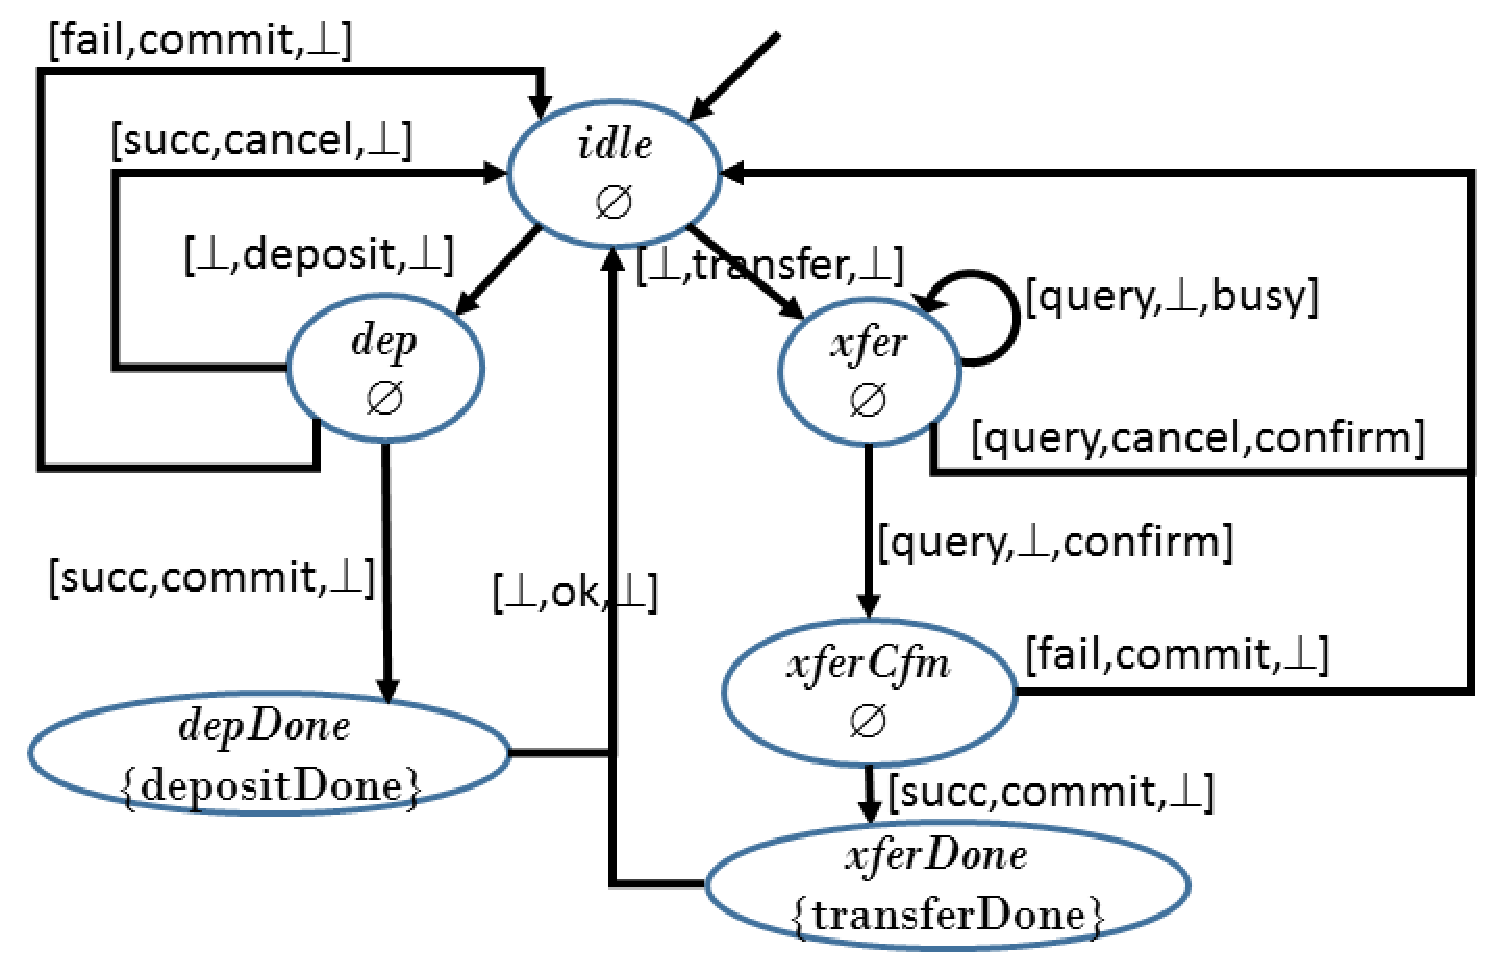
\epsfig{file=bank.eps,width=120mm} 
\caption{Game graph of a banking system} 
\label{fig.model.bank}
\end{center} 
\end{figure*} 
We need to find strategies of the agents to fulfill 
$\pfrr \neg \mbox{\sl checkOthersPassword}$, 
$\pevt \mbox{\sl depositDone}$, and 
$\pevt\mbox{\sl transferDone}$.  
To assist in our explanation of our verification algorithms, 
we use symbolic strategy names $x,y,z,w$ and the binding notations in formula (F).  
In fact, formula (G) is exactly the same as formula (E).  
Thus by interpreting all symbolic strategy names as existential quantified, 
formula (G) can be rewritten as follows.  
\begin{center} \hfill
$
\begin{array}{cl}
((1,x) \pfrr \neg \mbox{\sl checkOthersPassword}) \\
\wedge ((1,x)(2,y)\pevt \mbox{\sl depositDone}) \\
\wedge ((1,x)(2,z)(3,w)\pevt\mbox{\sl transferDone})
\end{array}
$
\hfill (H)
\end{center}   
Note that since we only allow explicit existential strategy quantification, 
the number of strategy bindings are exactly determined by the number and sizes of SQs and SIQs 
in the formula.  


If we label $(1,x) \pfrr \neg \mbox{\sl checkOthersPassword}$, $(1,x)(2,y)\pevt \mbox{\sl depositDone}$, and $(1,x)(2,z)$ $(3,w)\pevt\mbox{\sl transferDone}$ on nodes of a computation tree in a labelling procedure, then the symbolic names precisely reflect the the constraints on the decisions along plays. 
For example, suppose that both $(1,x) \pfrr \neg \mbox{\sl checkOthersPassword}$ and $(1,x)(2,y)\pevt \mbox{\sl depositDone}$ are labelled on a state of location {\em dep}. 
This state has three successor states: for convenience 
C1 of location {\em idle} via $[\mbox{\rm fail},\mbox{\rm commit},\perp]$, 
C2 of location {\em idle} via $[\mbox{\rm succ}, \mbox{\rm cancel}, \perp]$, and 
C3 of location {\em depDone} via $[\mbox{\rm succ}, \mbox{\rm commit}, \perp]$.  
If strategy $x$ chooses action succ, then obligation $(1,x) \pfrr \neg \mbox{\sl checkOthersPassword}$ will be passed down to C2 and C3.  
In this situation, whether obligation $(1,x)(2,y)\pevt \mbox{\sl depositDone}$ is labeled on C2 or C3 relies on the action decision of strategy $y$.  
But the constraint on strategy decision is that if $(1,x)(2,y)\pevt \mbox{\sl depositDone}$ is labeled on C2, then $(1,x) \pfrr \neg \mbox{\sl checkOthersPassword}$ must also be labeled on C2; and if  $(1,x)(2,y)\pevt \mbox{\sl depositDone}$ is labeled on C3, then $(1,x) \pfrr$ $\neg \mbox{\sl checkOthersPassword}$ must also be labeled on C3.  
The reason is that the path obligations are enforced by the same strategy of the bank.  

\subsection{Passing Down the Path Obligations While Observing the Restrictions Among S-Profiles}
The above observation points out how to judge whether a passing-down scheme of path obligations from a parent state to its child states are consistent with the strategy quantifications.  
For example, suppose that we have the following characteristics of the strategy profile $(1,x)(2,y)(2,z)(3,w)$.
\begin{list1} 
\item Strategy $x$ of the banking system never issues action fail. 
\item Strategy $y$ and $z$ never cancel transactions for its client. 
\item Strategy $w$ never shows busy message for the partner bank. 
\end{list1} 
Then the verification problem of strategy interaction can be visualized as finding strategies $x,y,z$, and $w$ that selecting paths in a computation tree to satisfy three path obligations: 
$\pfrr \neg \mbox{\sl checkOthersPassword}$, 
$\pevt \mbox{\sl depositDone}$, and $\pevt\mbox{\sl transferDone}$.  
Figure~\ref{fig.ctree} shows part of a computation tree when strategy $x$ for the banking system is fixed with the following restriction. 
\begin{figure*}[t] 
\begin{center} 
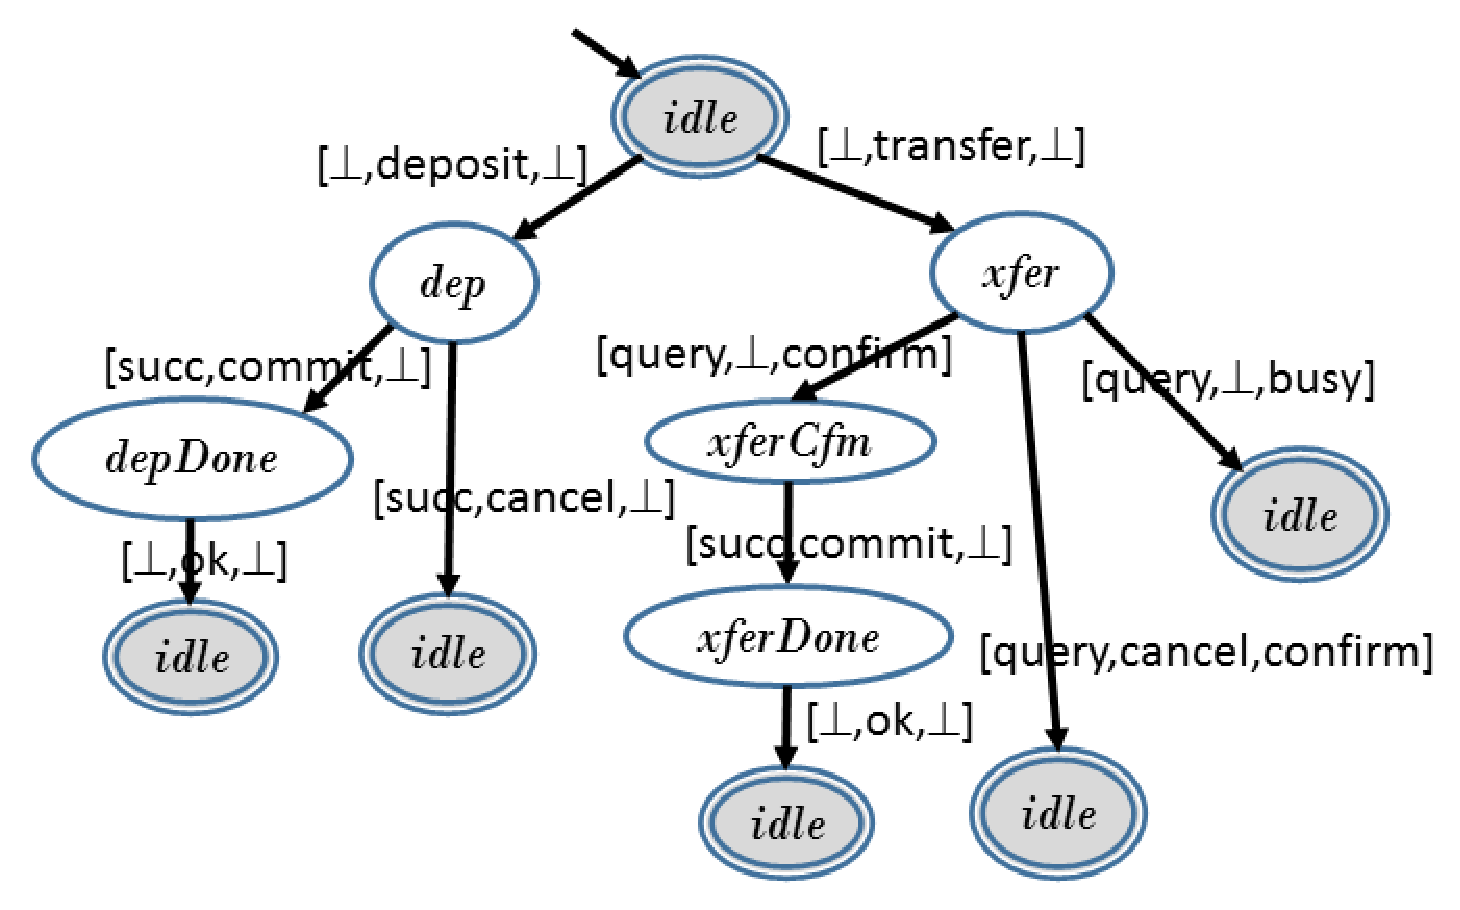
\epsfig{file=ctree.eps,width=120mm} 
\caption{Part of the computation tree of the banking system} 
\label{fig.ctree}
\end{center} 
\end{figure*} 
\begin{list1} 
\item At location {\em idle}, {\em depDone}, and {\em xferDone}, always issue action $\perp$.  
\item At location {\em dep} and {\em xferCfm}, only issue action {\sf succ}.  
\end{list1}
The leaves of the tree all end at location {\em idle} at which the same tree structure can be replicated.
We can start synthesizing strategy $y,z$, and $w$ in the context of this strategy $x$ which, for convenience of explanation, is memoryless (or positional). 

As we have suggested, we can label the path obligations on the nodes of the computation tree and examine whether a strategy profile can fulfill all the path obligations.
In the literature, we can name the nodes by their branching paths.
For example, the root is named $\varepsilon$ which is the empty string. 
Then the node at location {\em xferDone} is named '100' and 
the rightmost {\em idle} node is named '12.' 
We begin by label node `$\varepsilon$ with the three path obligations: 
$(1,x) \pfrr \neg \mbox{\sl checkOthersPassword}$, 
$(1,x)(2,y)\pevt \mbox{\sl depositDone}$, and $(1,x)(2,z)(3,w)$ $\pevt\mbox{\sl transferDone}$.  
Then we can pass the path obligations to the children in the following way. 
\begin{list1}
\item We must pass $(1,x) \pfrr \neg \mbox{\sl checkOthersPassword}$ to 
  both child '0' and '1' of the root since the two children 
  are both selected by action $\perp$ of the banking system. 
\item We can pass $(1,x)(2,y)\pevt \mbox{\sl depositDone}$ 
	and $(1,x)(2,z)(3,w)\pevt\mbox{\sl transferDone}$ respectively to 
	child '0' and '1' of the root since 
	the two children are selected with the same strategy $x$ of the banking system 
	and different strategies ($y$ and $z$) of the client.  
\end{list1} 
Note that we can check whether the passing down of the path obligation is consistent with the strategy quantifications in the input formula (G) just by checking the labelling of path obligations with strategy name bindings since all consistency information are maintained there.

Similarly, from node '0', strategy $x$ and $y$ can together choose to pass 
$(1,x)(2,y)\pevt$ $\mbox{\sl depositDone}$ to node '00' while strategy $x$ must unilaterally pass 
$(1,x) \pfrr \neg$ $\mbox{\sl checkOthersPassword}$ 
to both '00' and '01.'  
Then at node '00,' $(1,x)(2,y)\pevt \mbox{\sl depositDone}$ is fulfilled 
eventually and no longer need be passed down.  
The passing down of path obligations from node '1' and fulfillment of 
$(1,x)(2,z)(3,w)\pevt\mbox{\sl transferDone}$ can then be reasoned similarly.
 
\subsection{Finding Finite Satisfying Evidence for a Formula in a Computation Tree}
As we can see, the existence of the tree top in figure~\ref{fig.ctree} is sufficient for synthesizing strategy profile $(1,x)(2,y)(2,z)(3,w)$ to satisfy formula $(G)$.  
From this example, it is easy to see that the requirement for such a tree top.  
First, all eventual-formulas (or until-formulas) from the root SQ to the next level of SQs have to be fulfilled by the strategy profile.
Second, the leaves of the tree top do not contain any eventual-formula (or until-formula) labels.
Thus our PSPACE algorithm for model-checking BSIL formulas is actually a non-deterministic one that guess and check the consistency of the tree top and strategic actions at the nodes in the tree top.  

Then the final question regarding our algorithms is the terminating condition for searching the tree tops and strategy profiles.
Let us consider a tree node labelled with path obligations and how to (non-deterministically) explore for a tree top and a strategy profile.  
Note that the path obligations labelled on a child will be no more than those of its parent.  
In fact, the path obligations can stop being passed down in a path when it is fulfilled. 
Path obligations are simply passed down and not generated along the paths.  
As a result, along a path longer than the size of the game graph, either the number of path obligations decreases or two nodes, say $v$ and $v'$ 
(for convenience, we assume $v$ is an ancestor of $v'$), with identical location and labels must appear.
If the tree top is an evidence of existence of a strategy profile and the latter happens, then we can replace the the subtree rooted at $v$ with the one rooted at 
$v'$ and the result tree top is still an evidence.
This observation implies that we can focus on tree top such that along any path, no duplication of nodes with the same location and the same path obligation labels.  
This implies that we only have to explore tree tops of depth no greater than the size of the game graph times the number of temporal modalities in the given BSIL formula.


\section{BSIL}
\subsection{Syntax}
For concurrent game graph $\calg$ of $m$ agents, we have three types of formulas: {\em state formulas}, {\em tree formulas}, and {\em path formulas}.  
State formulas describe properties of states.  
Tree formulas describe interaction of strategies.  
Path formulas describe properties of plays.  
BSIL formulas are constructed with the following three syntax rules, 
respectively, for state formulas $\phi$, 
tree formulas $\tau$, and 
path formulas $\theta$.  
\begin{center}
$\begin{array}{rcl}
\phi    & ::= & p\;|\; \neg \phi_1 \;|\; \phi_1\vee \phi_2 
    \;|\; \langle  A\rangle \tau
    \;|\; \langle  A\rangle \theta
    \\
\tau  & ::= & \tau_1\vee \tau_2 \;|\; \tau_1\wedge \tau_2
    \;|\; \langle+ A\rangle \tau_1
    \;|\; \langle+ A\rangle\theta 
    \\
\theta  & ::= & \neg\theta_1 \;|\; \theta_1\vee \theta_2 
    \;|\; \nxt \phi_1
    \;|\; \phi_1\until \phi_2
\end{array}$
\end{center}
Here, $p$ is an atomic proposition in $P$ and
$A$ is an agency of $[1,m]$.
$\langle A\rangle$ is a {\em strategy quantifier} ({\em SQ}) and 
$\langle +A\rangle$ is a {\em strategy interaction quantifier} ({\em SIQ}).  
$\langle A\rangle\psi$ means that
there exists an S-profile for the agency $A$
that makes all plays satisfy $\psi$.
Formulas of the form $\langle+ B\rangle\psi_1$ must happen within an SQ.
Intuitively, they mean that there exists an S-profile of $B$
that collaborates with the strategies declared 
with ancestor formulas to make $\psi_1$ true. 
For convenience, we view SQs as special cases of SIQs. 
Also, for conciseness, we omit null SIQs $\langle+\rangle$.

State formulas $\phi$ are called {\em BSIL} {\em formulas}. 
From now on, we assume that we are always in the context of 
a given BSIL formula $\chi$.  
Note that we strictly require that strategy interaction cannot 
cross path modal operators.  
This restriction is important and allows us to analyze the interaction 
of strategies locally in a state and 
then enforce the interaction along all paths from this state.  

For convenience, we also use the common shorthands.
\begin{center} 
$
\true
\equiv p\vee(\neg p) 
\hspace*{10mm} 
\false
\equiv \neg\true 
\hspace*{10mm} 
\psi_1\Rightarrow \psi_2
\equiv (\neg \psi_1)\vee \psi_2$ \\
$\pevt \phi_1
\equiv \true\;\until \phi_1 
\hspace*{20mm} 
\pfrr \phi_1
\equiv \neg\pevt\neg\phi_1 
$
\end{center} 
The SQs and SIQs introduced above are 
all existential in that they are satisfied with one S-profile.  
Note that there is no universal SQs and SIQs in BSIL.  
This is purely for the complexity of the model-checking algorithm (and problem)
that we are going to present later.  
Thus BSIL can be used to specify the different ways of combining S-profiles 
to enforce system policy.  

For ease of notations, 
we may abbreviate 
$\langle \{a_1,\ldots,a_n\}\rangle$ and  
$\langle+ \{a_1,\ldots,a_n\}\rangle$ as 
$\langle a_1,\ldots,a_n\rangle$ and  
$\langle+a_1,\ldots,a_n\rangle$, respectively.
\subsection{semantics}
BSIL subformulas are interpreted with respect to S-profiles.  
A state or a tree formula $\phi$ is satisfied 
at a state $q$ with S-profile $\Sigma$, denoted $\calg,q\models_\Sigma\phi$, if,
and only if, the following inductive constraints are satisfied.
\begin{list1}
\item $\calg,q\models_\Sigma p$ iff $p\in \lambda(q)$.
\item For state formula $\phi_1$, 
    $\calg,q\models_\Sigma\neg\phi_1$ iff
    $\calg,q\models_\Sigma\phi_1$ is false.
\item For state or tree formulas $\psi_1$ and $\psi_2$, 
    $\calg,q\models_\Sigma\psi_1\wedge\psi_2$ iff
    $\calg,q\models_\Sigma\psi_1$
    and $\calg,q\models_\Sigma\psi_2$.
\item For state or tree formulas $\psi_1$ and $\psi_2$, 
    $\calg,q\models_\Sigma\psi_1\vee\psi_2$ iff
    either $\calg,q\models_\Sigma\psi_1$
    or $\calg,q\models_\Sigma\psi_2$.
\item $\calg,q\models_\Sigma\langle A\rangle\tau$
    iff there exists an S-profile $\Pi$ of $A$
    with $\calg,q\models_{\Pi}\tau$.  
\item $\calg,q\models_\Sigma\langle+A\rangle\tau$
    iff there exists an S-profile $\Pi$ of $A$
    with $\calg,q\models_{\Sigma\circ\Pi}\tau$.  
    Here, the composition $\Sigma\circ\Pi$ of the S-profiles $\Sigma$ and $\Pi$
    models the inheritance of 
    strategy bindings, $\Sigma$, from ancestor formulas. 
\item $\calg,q\models_\Sigma\langle A\rangle\theta$
    iff there exists an S-profile $\Pi$ of $A$ such that,
    for all plays $\rho$ from $q$ compatible with $\Pi$,
    $\rho\models_{\Pi}\theta$ holds.
    Intuitively, this means that $\rho$ satisfies path formula $\theta$ with S-profile $\Pi$.  
\item $\calg,q\models_\Sigma\langle + A\rangle\theta$
    iff there exists an S-profile $\Pi$ of $A$ such that, 
    for all plays $\rho$ from $q$ compatible with ${\Sigma\circ\Pi}$,
    $\rho\models_{\Sigma\circ\Pi}\theta$ holds.  
\end{list1} 

A play $\rho$ satisfies a path formula $\theta$ with S-profile $\Sigma$, 
in symbols $\rho\models_\Sigma\theta$, 
iff the following restrictions hold.
\begin{list1} 
\item For a path formula $\theta_1$, 
    $\rho\models_\Sigma\neg\theta_1$ iff
    it is not the case that $\rho\models_\Sigma\theta_1$.
\item For path formulas $\theta_1$ and $\theta_2$, 
    $\rho\models_\Sigma\theta_1\vee\theta_2$ iff
    either $\rho\models_\Sigma\theta_1$
    or $\rho\models_\Sigma\theta_2$.
\item $\rho\models_\Sigma\nxt\psi_1$
    iff $\calg,\rho(1)\models_\Sigma\psi_1$.
\item $\rho\models_\Sigma\psi_1\until\psi_2$
    iff there exists an $h\geq 0$ with $\calg,\rho(h)\models_\Sigma\psi_2$ 
    and for all $j\in [0,h)$, $\calg,\rho(j)\models_\Sigma\psi_1$.
\end{list1}
For convenience, we let $\perp$ be a null S-profile, 
i.e., a function that is undefined on everything. 
If $\phi_1$ is a BSIL (state) formula and $\calg,q\models_\perp\phi_1$,
then we may simply write $\calg,q\models\phi_1$.  
If $\calg,r\models\phi_1$, then we also write $\calg\models\phi_1$.
\subsection{ATL+}
ATL$^+$ is the syntactic fragment of BSIL given by the following grammar

\begin{center}
$\begin{array}{rcl}
\phi    & ::= & p\;|\; \neg \phi_1 \;|\; \phi_1\vee \phi_2 
    \;|\; \langle  A\rangle \theta
    \\
\theta  & ::= & \neg\theta_1 \;|\; \theta_1\vee \theta_2 
    \;|\; \nxt \phi_1
    \;|\; \phi_1\until \phi_2
\end{array}$
\end{center}

ATL$^+$ can also be viewed as an extension of ATL \cite{AHK02} that, similar to ...'s extension of CTL to CTL$^+$ \cite{BPM83,EH86}, allows for the Boolean combination of path formulas.
As such, all complexities of ATL$^+$ must reside between those of BSIL and ATL as well as between those of BSIL and CTL$^+$, which we will use to establish the lower bounds for ATL$^+$ and BSIL.

\subsection{Memory}
In this subsection, we show a simple example in which \label{reply1.in.which}  
the agents need memory to achieve their objective for ATL$^+$ 
specifications.
This is\label{reply1.is.is} exemplified by the simplest possible case: 
the turn based game in Figure~\ref{fig.gg.fin} 
with one agent, two states, one atomic proposition, 
and two memoryless strategies 
that do not count the unreached states in the histories.
For the ATL$^+$ sentence \label{reply2.mem.fin.parenthesis} 
$\langle 1 \rangle ((\neg \nxt p)\wedge \pevt p)$, 
apparently agent 1 needs memory to enforce it.  
\begin{figure}[t]
\begin{center} 
\begin{picture}(0,0)%
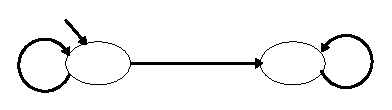
\includegraphics{gg.mem.fin60.eps}%
\end{picture}%
\setlength{\unitlength}{4144sp}%
%
\begingroup\makeatletter\ifx\SetFigFont\undefined%
\gdef\SetFigFont#1#2#3#4#5{%
  \reset@font\fontsize{#1}{#2pt}%
  \fontfamily{#3}\fontseries{#4}\fontshape{#5}%
  \selectfont}%
\fi\endgroup%
\begin{picture}(2724,580)(1631,299)
\put(2197,582){\makebox(0,0)[lb]{\smash{{\SetFigFont{7}{8.4}{\rmdefault}{\mddefault}{\updefault}{\color[rgb]{0,0,0}$v$}%
}}}}
\put(2197,445){\makebox(0,0)[lb]{\smash{{\SetFigFont{7}{8.4}{\rmdefault}{\mddefault}{\updefault}{\color[rgb]{0,0,0}$\emptyset$}%
}}}}
\put(3680,555){\makebox(0,0)[lb]{\smash{{\SetFigFont{7}{8.4}{\rmdefault}{\mddefault}{\updefault}{\color[rgb]{0,0,0}$u$}%
}}}}
\put(3652,418){\makebox(0,0)[lb]{\smash{{\SetFigFont{7}{8.4}{\rmdefault}{\mddefault}{\updefault}{\color[rgb]{0,0,0}$\{p\}$}%
}}}}
\end{picture}%

\end{center}
\caption{A simple turn-based game that demands memoryful strategies}
\label{fig.gg.fin}
\end{figure}

{\lemma \label{lemma.mem.fin}
The strategies of the agents in ATL$^+$ 
(and thus in BSIL) specifications need memory.
This even holds for the single agent case.
\qed 
}


\section{Expressive Power of BSIL}
In this section, we establish that BSIL is incomparable with ATL$^*$, 
AMC, and GL \cite{AHK02} in expressiveness.
In fact, we shall first establish the incomparability between BSIL with 
GL and AMC.  
Then the imcomparability with BSIL follows since GL and AMC are super-classes of 
ATL$^*$ \cite{AHK02}.
\subsection{Comparison with GL}
GL separates strategy quantifications\label{reply1.quantificaitons} from path quantifications.  
In comparison, ATL$^*$ and BSIL combines these two quantifications 
into SQs and SIQs.  
Thus with GL, we can specify that, for all S-profiles of $A$, 
there exists a play saitsfying $\psi_1$.  
The (existential) strategy quantification for agency $A$ 
of GL is of the form $\existsb A.\psi_1$.  
The path quantifications are just ordinary CTL modalities: 
$\forall\pfrr, \forall\until, \exists\pfrr$, and 
$\exists\until$.  

The following two lemmas show the relation between GL and BSIL.  
Lemma~\ref{lemma.gl.cant} uses two inductive families of game graphs 
to show that GL is not as expressive as BSIL. 
The base cases, $G_1$ and $H_1$, are in figure~\ref{fig.gg.exp}
for three agents.
\begin{figure}[t]\begin{center}
\begin{picture}(0,0)%
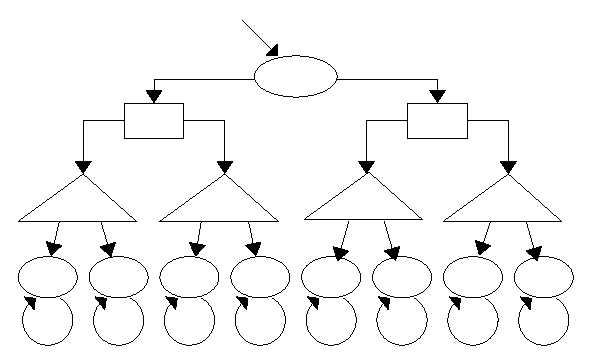
\includegraphics{gg.expba100.eps}%
\end{picture}%
\setlength{\unitlength}{4144sp}%
%
\begingroup\makeatletter\ifx\SetFigFont\undefined%
\gdef\SetFigFont#1#2#3#4#5{%
  \reset@font\fontsize{#1}{#2pt}%
  \fontfamily{#3}\fontseries{#4}\fontshape{#5}%
  \selectfont}%
\fi\endgroup%
\begin{picture}(4250,2496)(169,-1735)
\put(1396,-1276){\makebox(0,0)[lb]{\smash{{\SetFigFont{12}{14.4}{\rmdefault}{\mddefault}{\updefault}{\color[rgb]{0,0,0}$\{q\}$}%
}}}}
\put(3016,-1276){\makebox(0,0)[lb]{\smash{{\SetFigFont{12}{14.4}{\rmdefault}{\mddefault}{\updefault}{\color[rgb]{0,0,0}$\{q\}$}%
}}}}
\put(226,-1276){\makebox(0,0)[lb]{\smash{{\SetFigFont{12}{14.4}{\rmdefault}{\mddefault}{\updefault}{\color[rgb]{0,0,0}$\{p\}$}%
}}}}
\put(2566,-736){\makebox(0,0)[lb]{\smash{{\SetFigFont{12}{14.4}{\rmdefault}{\mddefault}{\updefault}{\color[rgb]{0,0,0}$\{p,q\}$}%
}}}}
\put(3646,-736){\makebox(0,0)[lb]{\smash{{\SetFigFont{12}{14.4}{\rmdefault}{\mddefault}{\updefault}{\color[rgb]{0,0,0}$\{p,q\}$}%
}}}}
\put(1486,-736){\makebox(0,0)[lb]{\smash{{\SetFigFont{12}{14.4}{\rmdefault}{\mddefault}{\updefault}{\color[rgb]{0,0,0}$\{p,q\}$}%
}}}}
\put(406,-736){\makebox(0,0)[lb]{\smash{{\SetFigFont{12}{14.4}{\rmdefault}{\mddefault}{\updefault}{\color[rgb]{0,0,0}$\{p,q\}$}%
}}}}
\put(2071,254){\makebox(0,0)[lb]{\smash{{\SetFigFont{12}{14.4}{\rmdefault}{\mddefault}{\updefault}{\color[rgb]{0,0,0}$\{p,q\}$}%
}}}}
\put(811,-1276){\makebox(0,0)[lb]{\smash{{\SetFigFont{12}{14.4}{\rmdefault}{\mddefault}{\updefault}{\color[rgb]{0,0,0}$\{p\}$}%
}}}}
\put(4051,-1276){\makebox(0,0)[lb]{\smash{{\SetFigFont{12}{14.4}{\rmdefault}{\mddefault}{\updefault}{\color[rgb]{0,0,0}$\{q\}$}%
}}}}
\put(1891,-1276){\makebox(0,0)[lb]{\smash{{\SetFigFont{12}{14.4}{\rmdefault}{\mddefault}{\updefault}{\color[rgb]{0,0,0}$\{q\}$}%
}}}}
\put(2431,-1276){\makebox(0,0)[lb]{\smash{{\SetFigFont{12}{14.4}{\rmdefault}{\mddefault}{\updefault}{\color[rgb]{0,0,0}$\{p\}$}%
}}}}
\put(3511,-1276){\makebox(0,0)[lb]{\smash{{\SetFigFont{12}{14.4}{\rmdefault}{\mddefault}{\updefault}{\color[rgb]{0,0,0}$\{p\}$}%
}}}}
\put(3151,-61){\makebox(0,0)[lb]{\smash{{\SetFigFont{12}{14.4}{\rmdefault}{\mddefault}{\updefault}{\color[rgb]{0,0,0}$\{p,q\}$}%
}}}}
\put(991,-61){\makebox(0,0)[lb]{\smash{{\SetFigFont{12}{14.4}{\rmdefault}{\mddefault}{\updefault}{\color[rgb]{0,0,0}$\{p,q\}$}%
}}}}
\put(2341,524){\makebox(0,0)[lb]{\smash{{\SetFigFont{12}{14.4}{\rmdefault}{\mddefault}{\updefault}{\color[rgb]{0,0,0}$r_0$}%
}}}}
\end{picture}%
\\
(a) $G_1$, a game graph for base case.\\
\begin{picture}(0,0)%
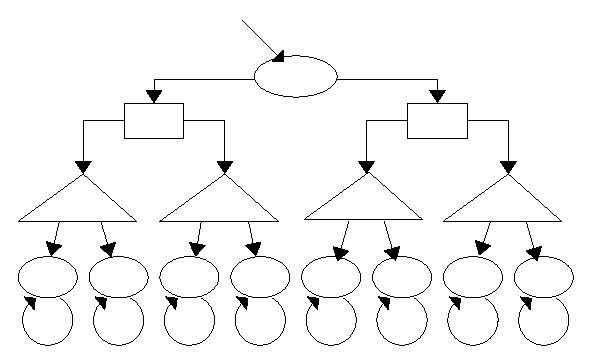
\includegraphics{gg.expbb100.eps}%
\end{picture}%
\setlength{\unitlength}{4144sp}%
%
\begingroup\makeatletter\ifx\SetFigFont\undefined%
\gdef\SetFigFont#1#2#3#4#5{%
  \reset@font\fontsize{#1}{#2pt}%
  \fontfamily{#3}\fontseries{#4}\fontshape{#5}%
  \selectfont}%
\fi\endgroup%
\begin{picture}(4250,2496)(169,-1735)
\put(856,-1276){\makebox(0,0)[lb]{\smash{{\SetFigFont{12}{14.4}{\rmdefault}{\mddefault}{\updefault}{\color[rgb]{0,0,0}$\{p\}$}%
}}}}
\put(1396,-1276){\makebox(0,0)[lb]{\smash{{\SetFigFont{12}{14.4}{\rmdefault}{\mddefault}{\updefault}{\color[rgb]{0,0,0}$\{p\}$}%
}}}}
\put(3016,-1276){\makebox(0,0)[lb]{\smash{{\SetFigFont{12}{14.4}{\rmdefault}{\mddefault}{\updefault}{\color[rgb]{0,0,0}$\{q\}$}%
}}}}
\put(3556,-1276){\makebox(0,0)[lb]{\smash{{\SetFigFont{12}{14.4}{\rmdefault}{\mddefault}{\updefault}{\color[rgb]{0,0,0}$\{p\}$}%
}}}}
\put(226,-1276){\makebox(0,0)[lb]{\smash{{\SetFigFont{12}{14.4}{\rmdefault}{\mddefault}{\updefault}{\color[rgb]{0,0,0}$\{p\}$}%
}}}}
\put(2566,-736){\makebox(0,0)[lb]{\smash{{\SetFigFont{12}{14.4}{\rmdefault}{\mddefault}{\updefault}{\color[rgb]{0,0,0}$\{p,q\}$}%
}}}}
\put(3646,-736){\makebox(0,0)[lb]{\smash{{\SetFigFont{12}{14.4}{\rmdefault}{\mddefault}{\updefault}{\color[rgb]{0,0,0}$\{p,q\}$}%
}}}}
\put(1486,-736){\makebox(0,0)[lb]{\smash{{\SetFigFont{12}{14.4}{\rmdefault}{\mddefault}{\updefault}{\color[rgb]{0,0,0}$\{p,q\}$}%
}}}}
\put(406,-736){\makebox(0,0)[lb]{\smash{{\SetFigFont{12}{14.4}{\rmdefault}{\mddefault}{\updefault}{\color[rgb]{0,0,0}$\{p,q\}$}%
}}}}
\put(2071,254){\makebox(0,0)[lb]{\smash{{\SetFigFont{12}{14.4}{\rmdefault}{\mddefault}{\updefault}{\color[rgb]{0,0,0}$\{p,q\}$}%
}}}}
\put(4051,-1276){\makebox(0,0)[lb]{\smash{{\SetFigFont{12}{14.4}{\rmdefault}{\mddefault}{\updefault}{\color[rgb]{0,0,0}$\{q\}$}%
}}}}
\put(3151,-106){\makebox(0,0)[lb]{\smash{{\SetFigFont{12}{14.4}{\rmdefault}{\mddefault}{\updefault}{\color[rgb]{0,0,0}$\{p,q\}$}%
}}}}
\put(991,-106){\makebox(0,0)[lb]{\smash{{\SetFigFont{12}{14.4}{\rmdefault}{\mddefault}{\updefault}{\color[rgb]{0,0,0}$\{p,q\}$}%
}}}}
\put(1891,-1276){\makebox(0,0)[lb]{\smash{{\SetFigFont{12}{14.4}{\rmdefault}{\mddefault}{\updefault}{\color[rgb]{0,0,0}$\{q\}$}%
}}}}
\put(2431,-1276){\makebox(0,0)[lb]{\smash{{\SetFigFont{12}{14.4}{\rmdefault}{\mddefault}{\updefault}{\color[rgb]{0,0,0}$\{q\}$}%
}}}}
\put(2296,524){\makebox(0,0)[lb]{\smash{{\SetFigFont{12}{14.4}{\rmdefault}{\mddefault}{\updefault}{\color[rgb]{0,0,0}$s_0$}%
}}}}
\end{picture}%
\\
(b) $H_1$, another game graph for base case.\\
$\bigcirc$ belongs to Agent  1; $\pfrr$ belongs to Agent 2; and 
$\triangle$ belongs to Agent 3.
\end{center}
\caption{Base cases for the expressiveness of BSIL over ATL$^*$}
\label{fig.gg.exp}
\end{figure}
The inductive cases, $G_{k+1}$ and $H_{k+1}$, are 
respectively constructed out of $G_k$ and $H_k$ as 
in figure~\ref{fig.gg.expi}.
\begin{figure}[t]\begin{center}
\begin{picture}(0,0)%
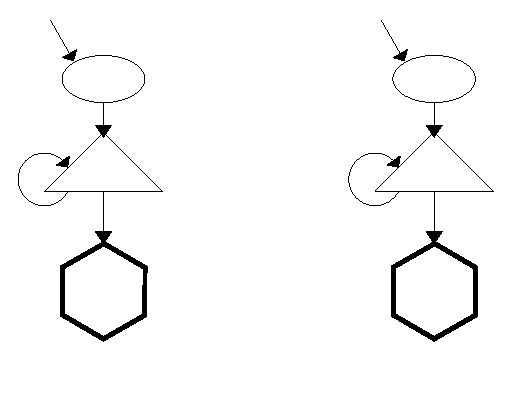
\includegraphics{gg.expi100.eps}%
\end{picture}%
\setlength{\unitlength}{4144sp}%
%
\begingroup\makeatletter\ifx\SetFigFont\undefined%
\gdef\SetFigFont#1#2#3#4#5{%
  \reset@font\fontsize{#1}{#2pt}%
  \fontfamily{#3}\fontseries{#4}\fontshape{#5}%
  \selectfont}%
\fi\endgroup%
\begin{picture}(3643,2925)(1635,-2164)
\put(1891,-2086){\makebox(0,0)[lb]{\smash{{\SetFigFont{12}{14.4}{\rmdefault}{\mddefault}{\updefault}{\color[rgb]{0,0,0}(a) $G_k$}%
}}}}
\put(4411,-2086){\makebox(0,0)[lb]{\smash{{\SetFigFont{12}{14.4}{\rmdefault}{\mddefault}{\updefault}{\color[rgb]{0,0,0}(b) $H_k$}%
}}}}
\put(2116,-1366){\makebox(0,0)[lb]{\smash{{\SetFigFont{12}{14.4}{\rmdefault}{\mddefault}{\updefault}{\color[rgb]{0,0,0}$G_{k-1}$}%
}}}}
\put(4636,-1366){\makebox(0,0)[lb]{\smash{{\SetFigFont{12}{14.4}{\rmdefault}{\mddefault}{\updefault}{\color[rgb]{0,0,0}$H_{k-1}$}%
}}}}
\put(2071,-466){\makebox(0,0)[lb]{\smash{{\SetFigFont{12}{14.4}{\rmdefault}{\mddefault}{\updefault}{\color[rgb]{0,0,0}$\{p,q\}$}%
}}}}
\put(4591,-466){\makebox(0,0)[lb]{\smash{{\SetFigFont{12}{14.4}{\rmdefault}{\mddefault}{\updefault}{\color[rgb]{0,0,0}$\{p,q\}$}%
}}}}
\put(4591,254){\makebox(0,0)[lb]{\smash{{\SetFigFont{12}{14.4}{\rmdefault}{\mddefault}{\updefault}{\color[rgb]{0,0,0}$\{p,q\}$}%
}}}}
\put(2071,254){\makebox(0,0)[lb]{\smash{{\SetFigFont{12}{14.4}{\rmdefault}{\mddefault}{\updefault}{\color[rgb]{0,0,0}$\{p,q\}$}%
}}}}
\put(2251,524){\makebox(0,0)[lb]{\smash{{\SetFigFont{12}{14.4}{\rmdefault}{\mddefault}{\updefault}{\color[rgb]{0,0,0}$r_k$}%
}}}}
\put(4816,524){\makebox(0,0)[lb]{\smash{{\SetFigFont{12}{14.4}{\rmdefault}{\mddefault}{\updefault}{\color[rgb]{0,0,0}$s_k$}%
}}}}
\end{picture}%
\\
$\bigcirc$ belongs to Agent  1; $\pfrr$ belongs to Agent 2; and 
$\triangle$ belongs to Agent 3.
\end{center}
\caption{Inductive cases for the expressiveness of BSIL over ATL$^*$}
\label{fig.gg.expi}
\end{figure}


{\lemma \label{lemma.gl.cant}
Every GL formula $\phi$ with $k$ ($k>0$) SQs cannot distinguish 
$G_k$ and $H_k$ while 
$\langle 1\rangle ((\langle+ 2\rangle\pfrr p)
    \wedge \langle+ 2\rangle\pfrr q)$ can.
}
\\\pf 
It is clear that
$\langle 1\rangle ((\langle+ 2\rangle \pfrr p)
    \wedge (\langle+ 2\rangle \pfrr q))$ can $G_k$ and $H_k$ 
no matter what value $k$ is.  
The proof continues by an induction $k$, the numbrer of SQs in $\phi$. 

\noindent 
{\bf Base case:} Assume that $\phi$ has only one modal operator.
Then there are the following case analysis of GL formulas.
\begin{list1}
\item {\bf Case 1:} {\em $\phi$ is $\existsb  A.\phi_1$
    where $\phi_1$ is a Boolean combination of
    formulas of the form $\exists \psi$ or $\forall \psi$
    where $\psi$ is a path formula.}
    Note that $\phi_1$ characterizes a set of states that 
    either start a play satisfying $\psi$ or 
    start only plays satisfying $\psi$.
    The following case analysis shows that, for every
    trace subset $S$ and every agency $A$,
    there exists a strategy of $A$ to characterize
    $S$ in figure~\ref{fig.gg.exp}(a) iff
    there exists a strategy for $A$ to characterize
    $S$ in figure~\ref{fig.gg.exp}(b).
    \begin{list2}
    \item {\bf Case 1a:} {\em $\phi$ is $\existsb\emptyset.\phi_1$.}
        In this case, there is no strategy and the sets of traces
        imposed by no strategy in the two state graphs are
        both $\{\pfrr p,\pfrr q\}$.
        Thus, $\existsb\emptyset.\phi_1$ cannot distinguish the trace sets of the
        two state graphs.
    \item {\bf Case 1b:} {\em $\phi$ is $\existsb\{1\}.\phi_1$.}
        From figure~\ref{fig.gg.exp}, no matter what strategies
        agency $\{1\}$ may choose, the
        trace sets for the two game graphs are both
        $\{\pfrr p,\pfrr q\}$.
        Thus, $\existsb\{1\}.\phi_1$ cannot distinguish the trace sets of the
        two state graphs.
    \item {\bf Case 1c:} {\em $\phi$ is
        $\existsb\{2\}.\phi_1$.}
        This case is similar to case 1b.
    \item {\bf Case 1d:} {\em $\phi$ is
        $\existsb\{3\}.\phi_1$.}
        This case is similar to case 1b.
    \item {\bf Case 1e:} {\em $\phi$ is
        $\existsb\{1,2\}.\phi_1$.}
        Agency $\{1, 2\}$ can cooperate to force three trace sets:
        $\{\pfrr p\}, \{\pfrr q\}, \{\pfrr p,\pfrr q\}$
        in both of the game graphs in figure~\ref{fig.gg.exp}.
        Thus, $\existsb\{1,2\}.\phi_1$ cannot distinguish the trace sets of the
        two state graphs.
    \item {\bf Case 1f:} {\em $\phi$ is
        $\existsb\{1,3\}.\phi_1$.}
        This case is similar to case 1e.
    \item {\bf Case 1g:} {\em $\phi$ is
        $\existsb\{2,3\}.\phi_1$.}
        This case is similar to case 1e.
    \item {\bf Case 1h:} {\em $\phi$ is
        $\existsb\{1,2,3\}.\phi_1$.}
        Agency $\{1, 2,3\}$ can cooperate to force three trace sets:
        $\{\pfrr p\}, \{\pfrr q\}, \{\pfrr p,\pfrr q\}$
        in both of the game graphs in figure~\ref{fig.gg.exp}.
        Thus, $\existsb\{1,2,3\}.\phi_1$ cannot distinguish the trace sets of the
        two state graphs.
    \end{list2}
\item {\bf Case 2:} {\em $\phi$ is a Boolean combination of
    formulas in case 1.}
    Since case 1 does not distinguish the two game graphs, 
    this case can neither do it.  
\end{list1}
Thus the base case is proven.

\noindent {\bf Induction step:}
If $\phi$ has $k$ modal operators,
to tell the difference between $G_k$ and $H_k$,
we need a modal subformula of $\phi$ that can tell the difference
of $G_{k-1}$ and $H_{k-1}$.
But according to the inductive hypothesis, this is impossible.
Thus the lemma is proven.  
\qed 



{\lemma \label{lemma.gl.incomp}
GL formula $\existsb\{1\}.((\exists\pfrr p)\wedge\exists\pfrr q)$
is not equivalent to any BSIL formula.
}
\\\pf The proof basically follows the same argument in \cite{AHK02} 
that $\existsb\{1\}.((\exists\pfrr p)\wedge\exists\pfrr q)$ 
is not equivalent to 
any ATL$^*$ formula.  
\qed 

Lemmas~\ref{lemma.gl.cant} and 
\ref{lemma.gl.incomp} together show that 
GL and BSIL are not comparable in expressiveness.  
\subsection{Comparison with AMC}
AMC is an extension from $\mu$-calculus and allows 
for multiple fixpoints interleaved together \cite{AHK02}.  
An AMC formula contains fixpoint operators on state set variables.  
The only modality of AMC is of the form $\langle A\rangle\nxt\psi$ 
and least fixpoint $\emlfp x.\psi_1(x)$ where 
$\psi_1(x)$ is a Boolean function of atomic propositions 
and state set variables (including $x$).  
It is required that every occurrence of $x$ in $\psi_1$ is 
under even number of negations.  
The duality of the least fixpoint operator is the greatest fixpoint 
operator $\emgfp$.  
Formula $\emgfp x.\psi_1$ is defined as $\neg\emlfp x.\neg\psi_1(x)$.  

To establish that AMC is not as expressive as BSIL, we basically follow 
the proof style for Lemma~\ref{lemma.atl.cant} and 
use the same two families of game graphs.  
% (See appendix~\ref{app.lemma.atl.cant}).  
The statement of the lemma requires notations for 
state set variables and other details in AMC. 
We need to define the domain of values for the free state set variables 
in AMC formulas.  
Let $X$ be the set of state set variables.  
Without loss of generality, we assume that no two subformulas
of the form $\emlfp x.\phi$ in
a given AMC formula share the same quantified name of $x$.
Given a subformula $\emlfp x_i.\phi$
with free variables $x_1,\ldots,x_n$ in $\phi$
and no modal operator $\langle\ldots\rangle\nxt$ in $\phi$,
we define $\phi$ as a {\em base template} for $x_i$.
Then we can define the {\em base formula domain} of $x_i$,
denoted $F_0(x_i)$,
as the smallest set with the following restrictions.
We let $\phi[x_1\mapsto \eta_1,\ldots,x_n\mapsto\eta_n]$ 
be the AMC formula identical to 
$\phi$ except that every occurrence of $x_i$ in $\phi$ are respectively 
replaced with $\eta_i$.  
\begin{list1}
\item For each $x_i\in X$ with base template $\phi$,
    $\phi[x_1\mapsto\false,\ldots,x_n\mapsto\false]\in F_0(x_i)$.
\item For each $x_i\in X$ with base template $\phi$
    and $\phi_1\in F_0(x_1),\ldots,\phi_n\in F_0(x_n)$,
    $\phi[x_1\mapsto\phi_1,\ldots,x_n\mapsto\phi_n]\in F_0(x_i)$.
\end{list1}
Note that there is neither variables nor `$\emlfp$' operators
in $F_0(x)$ for every $x$.
Thus we can define the characterization $\kappa$ 
of a formula $\phi_1$ in $F_0(x)$ for $\calg$,
in symbols $\kappa(\calg,\phi_1)$, as follows.
\begin{list1}
\item For each atomic proposition $p\in P$,
    $\kappa(\calg,p)=\{q\mid p\in\lambda(q)\}$.
\item For each $\phi\in F_0(x)$, 
    $\kappa(\calg,\neg\phi)=Q-\kappa(\calg,\phi)$.
\item For each $\phi_1,\phi_2\in F_0(x)$,
    $\kappa(\calg,\phi_1\vee\phi_2)=\kappa(\calg,\phi_1)\cup\kappa(\calg,\phi_2)$.
\end{list1}
A {\em valuation} $\nu$ of variables in $X$ for $\calg$
is a mapping from
$X$ such that, for each $x\in X$, there exists a base domain formula
$\phi$ of $x$ such that $\nu(x)= \kappa(\calg,\phi)$.

The expressiveness comparison between AMC and BSIL relies on the
following lemma.

{\lemma \label{lemma.amc.domain}
For every AMC formula $\phi$ without modal operator of the
form $\langle\ldots\rangle\nxt$, state set variable $x$, and
a formula $\phi_1$ in $F_0(x)$,
$r_0\in\kappa(G_0,\phi_1)$
iff
$s_0\in\kappa(H_0,\phi_1)$
in figure~\ref{fig.gg.exp}.
}
\\\pf 
We can prove this with an structural induction on $\phi_1$.
The base case is straightforward.
The inductive step follows since Boolean combinations of
subformulas that cannot distinguish $G_0$ and $H_0$ can neither
distinguish the two game graphs.
\qed


Now we want to classify AMC formulas according to the nesting depths of
operators of the form $\langle\ldots\rangle\nxt$ in a formula.
Specifically, we let $\mbox{AMC}^{(k)}$ be the set of AMC formulas
with exactly nesting depth $k$ of operator $\langle \ldots\rangle\nxt$.
For example,
$\emlfp x.\langle 1\rangle \nxt
(p\rightarrow \emlfp y.\langle 2\rangle (x\vee y\wedge\nxt q))$
is in $\mbox{AMC}^{(2)}$.
Then, $\mbox{AMC}^{(0)}$ is
the smallest set with the following restrictions.
\begin{list1}
\item {\bf Case 1a:} For each atomic proposition $p\in P$,
    $p\in \mbox{AMC}^{(0)}$.
\item {\bf Case 1b:} For each proposition variable $x\in X$,
    $x\in \mbox{AMC}^{(0)}$.
\item {\bf Case 1c:} For each $\phi\in \mbox{AMC}^{(0)}$,
    $\neg\phi\in \mbox{AMC}^{(0)}$.
\item {\bf Case 1d:} For each $\phi_1,\phi_2\in \mbox{AMC}^{(0)}$,
    $\phi_1\vee\phi_2\in \mbox{AMC}^{(0)}$.
\item {\bf Case 1e:} For each $\phi\in \mbox{AMC}^{(0)}$ and
    proposition variable $x\in X$,
    $\emlfp x.\phi\in \mbox{AMC}^{(0)}$.
\end{list1}
Then $\mbox{AMC}^{(k)}$, $k>0$,
is the smallest set with the following restrictions.
\begin{list1}
\item {\bf Case 2a:} For each $A\subseteq [1,m]$ and
    $\phi\in \mbox{AMC}^{(k-1)}$,
    $\langle A\rangle \nxt \phi\in \mbox{AMC}^{(k)}$,
\item {\bf Case 2b:} For each $\phi\in \mbox{AMC}^{(k)}$,
    $\neg\phi\in \mbox{AMC}^{(k)}$.
\item {\bf Case 2c:} For each $\phi_1\in \mbox{AMC}^{(k)}$ and
    $\phi_2\in\bigcup_{h\leq k}\mbox{AMC}^{(h)}$,
    $\phi_1\vee\phi_2\in \mbox{AMC}^{(k)}$.
\item {\bf Case 2d:} For each
    $\phi_1\in\bigcup_{h\leq k}\mbox{AMC}^{(h)}$ and $\phi_2\in \mbox{AMC}^{(k)}$,
    $\phi_1\vee\phi_2\in \mbox{AMC}^{(k)}$.
\item {\bf Case 2e:} For each $\phi\in \mbox{AMC}^{(k)}$ and
    proposition variable $x\in X$,
    $\emlfp x.\phi\in \mbox{AMC}^{(k)}$.
\end{list1}
Note that there could be free variables in the formulas classified in
the above.
The evaluation of such formulas for a game graph depends on the
valuation of the free variables.

Given two game graphs $G,H$ and
an AMC formulas $\phi$,
we say that
two valuations of $\nu$ and $\nu'$ respectively of $G$ and $H$
are {\em consistent} if for every $x\in X$,
there exists a $\phi_1\in F_0(x)$ such that
$\nu(x)=\kappa(G,\phi_1)$ and $\nu'(x)=\kappa(H,\phi_1)$.
In the following, we adopt the AMC semantic notations in \cite{AHK02}.
Given a game graph $G$, an AMC formula $\phi$,
and a valuation $\nu$ of state set variables in $X$,
$(\phi)^G(\nu)$ denotes the set of states of $G$ that
satisfy $\phi$ with valuation $\nu$.







{\lemma\label{lemma.amc.induction}
Assume that $G_k$ and $H_k$ are defined in
figures~\ref{fig.gg.exp} and \ref{fig.gg.expi}.
For every $k$, AMC formula $\phi\in \mbox{AMC}^{(k)}$, and two consistent
valuations $\nu$ and $\nu'$ respectively of $G_k$ and $H_k$,
$r_k\in (\phi)^{G_k}(\nu)$ iff
$s_k\in (\phi)^{H_k}(\nu')$.
}
\\\pf
We use an induction on $k$ to prove the lemma.

\noindent
{\bf Base case:} 
When $\phi$ is in case 1a through 1d, the lemma follows straightforwardly.
In case 1e,
$(\emlfp x.\psi)^{G_1}(\nu)$ can be expanded as follows.
We let
\begin{list1}
\item $\psi^{G_1,\nu,(0)}$ be $(\psi[x\mapsto \false])^{G_1}(\nu)$ and
\item for each $h>0$,
    $\psi^{G_1,\nu,(h)}$ be $(\phi[x\mapsto \psi_1^{G_1,(h-1)}])(\nu)$.
\end{list1}
Then $(\emlfp x.\phi)^{G_1}(\nu)=\bigcup_{h\geq 0}\psi^{G_1,\nu,(h)}$
according to the semantics of AMC.
Similarly, \linebreak 
$(\emlfp x.\phi)^{H_1}(\nu')=\bigcup_{h\geq 0}\psi^{H_1,\nu',(h)}$.
According to the same argument for cases 1a through 1d,
for each $h\geq 0$,
$r_0\in \psi^{G_1,\nu,(h)}$ iff
$s_0\in \psi^{H_1,\nu',(h)}$.
Thus it is clear that
$r_0\in (\emlfp x.\phi)^{G_1}(\nu)$ iff
$s_0\in (\emlfp x.\phi)^{H_1}(\nu')$.
Thus the lemma is proven in this case.

\noindent
{\bf Induction step:}
To tell the difference between $G_k$ and $H_k$,
we need a formula with the following structure.
\begin{list1}
\item At least one nesting of operators
    like $\langle\ldots\rangle\nxt$ in a least fixpoint operation 
    to infer the reachability of $G_{k-1}$ and $H_{k-1}$.
\item A modal subformula nested inside a $\langle \ldots\rangle \nxt$
    modal operator of $\phi$ that can tell the difference
    of $G_{k-1}$ and $H_{k-1}$.  
    But according to the inductive hypothesis, this is impossible.  
\end{list1}
Thus the lemma is proven.
\qed


Then with Lemma~\ref{lemma.amc.induction}, 
we conclude the proof for Lemma~\ref{lemma.amc.cant} in the following. 


{\lemma \label{lemma.amc.cant}
For every AMC formula $\phi$,
there are two game graphs that
$\phi$ cannot distinguish while
$\langle 1\rangle ((\langle+ 2\rangle\pfrr p)
    \wedge \langle+ 2\rangle\pfrr q)$ can.
}
\\\pf 
In the proof for Lemma~\ref{lemma.amc.induction}, 
it is apparent that $\phi$ with $\phi\in\mbox{AMC}^{(k)}$ cannot 
tell $G_k$ and $H_k$.  
\qed 

By the same argument in \cite{AHK02}, 
for one-agent game, BSIL coincides with CTL and is not as expressive as 
AMC. 

{\lemma \label{lemma.amc.can}
For game graphs of one agent,
AMC is strictly more expressive than BSIL.} 
\\\pf 
For one-agent games, 
AMC is equivalent to $\mu$-calculus and BSIL is equivalent to CTL which
is strictly less expressive than $\mu$-calculus.
\qed 



A comment on Lemmas~\ref{lemma.gl.cant} and \ref{lemma.amc.cant} 
is that the path modal formulas in the lemmas can be changed 
independently to $\pevt \neg p$ and $\pevt \neg q$ without affecting the validity of 
the lemma.  
This can be used to show that the example properties in the introduction 
are indeed inexpressible in ATL$^*$, GL, and AMC.  

\subsection{Comparison with ATL*}
It is easy to see that BSIL is a super-class of ATL.
Thus we have the following lemma.

{\lemma \label{lemma.atl.less}
BSIL is at least as expressive as ATL.  
}
% \\\pf The lemma is true since BSIL without SIQs coincides with ATL.  
\qed

Then Lemmas~\ref{lemma.gl.cant} and \ref{lemma.amc.cant} 
lead to the 
fact that there are some BSIL properties that 
ATL$^*$ cannot express 
since GL and AMC are both super-class of ATL$^*$ \cite{AHK02}.  



{\lemma \label{lemma.atl.cant} 
For every ATL$^*$ formula $\phi$, 
there are two game graphs that
$\phi$ cannot distinguish while
$\langle 1\rangle ((\langle+ 2\rangle\pfrr p)
    \wedge \langle+ 2\rangle\pfrr q)$ can.
}\qed 

Lemmas~\ref{lemma.atl.less} and \ref{lemma.atl.cant} together establish  
that ATL is strictly less expressive than BSIL. 
Then the following lemma shows the reverse direction.  

{\lemma \label{lemma.atl.incomp}
ATL$^*$ formula $\langle 1\rangle\pfrr\pevt p$
is not equivalent to any BSIL formula.
} 
\\\pf 
The proof is similar to the proof for the inexpressibility of 
$\langle 1\rangle\pfrr\pevt p$ with ATL \cite{AHK02}.  
\qed 

Lemmas~\ref{lemma.atl.cant} and \ref{lemma.atl.incomp}
together establish  
that ATL$^*$ and BSIL are not comparable in expressiveness. 

\section{Algorithm and Complexity}
The model-checking problem of BSIL is contained in 
PSPACE mainly due to the restriction that disallows 
negation in tree formulas.
As in the model-checking algorithms 
of ATL \cite{AHK02}, we can evaluate the proper state subformulas \label{reply1.subformulas.formulas} 
independently and then treat them as auxiliary propositions.  
Moreover, as in the evaluation of $\pevt$-formulas in 
ATL model-checking, 
if a $\pevt$-formula can be enforced with an S-profile, it can be enforced 
in a finite number of steps along every play compatible with 
the strategy in a computation tree.  
Once a bound $b$ for this finite number of steps is determined, 
we can enumerate all strategies embedded in the computation 
tree up to depth $b$ and try to find one that enforces a BSIL formula.  

\label{reply2.exp.alg2} 
As explained in section~\ref{sec.running}, 
our algorithm also labels subformulas and their symbolic S-profiles 
on the nodes in a computation tree. 
The formula is satisfied if and only if we can 
find a finite tree top with labels consistent with the SQs and SIQs in the input formula 
and can be extended to an infinite computation tree. 
In Subsection~\ref{subsec.children.ltl.ob},
we derive the labels, i.e., subformulas and their symbolic S-profiles, that are 
sufficient for our model-checking algorithm and 
present two procedures: 
\begin{list1} 
\item \tteval() that checks whether the satisfaction of formulas at a state 
	can be decided locally.  
\item \ttsynsuc() that nondeterministically chooses a scheme to 
	pass down the subformulas and their symbolic S-profiles to the child nodes 
	without violating the restrictions on the S-profiles declared with the SQs and SIQs. 
\end{list1} 

There are, however, severe differences between exploring 
a computation tree for 
BSIL and exploring one for ATL \cite{AHK02}.   
For BSIL, we have to take the interaction of strategies into account.  
For example, we may have to enforce a subformula 
$\langle 1\rangle((\langle+ 2\rangle \pevt p)
\wedge\langle+ 2\rangle (\pfrr q\vee \pevt r))$.  
Then, when exploring the computation tree, 
we may follow two strategies of Agent 2, one to enforce $\pevt p$ and 
the other to enforce $\pfrr q$ or $\pevt r$.  
There are the following situation for the 
interaction between these two strategies. 
The two strategies may make the same decision all the way 
until we reach a tree node $v$.  
(For turn-based games, $v$ has to be owned by Agent 2.)    
This can be conceptualized as passing the obligations of $\pevt p$ and 
$\pfrr q\vee\pevt r$ along the path from the root to $v$.  
Then, at node $v$, the two strategies may differ in their decisions 
and pass down the two obligations to different branches. 

\label{reply2.exp.alg3} 
Then, in Subsection~\ref{subsec.alg.proc},
we present our algorithm in two parts,
one for model-checking BSIL state formulas
and the other for model-checking BSIL tree formulas.
In Subsection~\ref{subsec.alg.corr},
we prove the correctness of the algorithm.
In Subsection~\ref{subsec.alg.pspace}, 
we show that our algorithm is in PSPACE.  
Together with Lemma~\ref{lemma.bsil.mck.nphard} in 
Subsection~\ref{subsec.pspace.hard}, 
we then establish the PSPACE-completeness of 
the BSIL and ATL$^+$ model-checking problems.  



\subsection{Computing path obligations and passing them down the computation tree
\label{subsec.children.ltl.ob}
}

We use $\{a_1 \mapsto s_1,\ldots,a_n\mapsto s_n\}$ to denote 
a partial function that maps $a_i$ to $s_i$ for each $i\in[1,n]$.  
Given a partial function $f$, 
we denote the domain of $f$ by $\emdef(f)$.
Inheriting the notations in \cite{MMV10}, 
we may also represent the the mapping as $(a_1,s_1)(a_2,s_2)\ldots(a_n,s_n)$.  
% be the set of domain elements that 
% is defined with $\zeta$.  

We need some special techniques in checking tree formulas.  
We adopt the concept of strategy variables from \cite{CHP10,MMV10}. 
A {\em strategy variable binding} ({\em SV-binding} for short) 
is a partial function from $[1,m]$ to strategy variables.  
Given an SV-binding $\Lambda$, 
$\Lambda\circ(a_1, s_1)\ldots(a_n, s_n)$ 
is the SV-binding that is identical to $\Lambda$ 
except that Agent $a_i$ is bound to $s_i$ for every $i\in[1,n]$.  
% Given an agency $A\subseteq[1,m]$, 
% $\Lambda^{\neg A}$ is defined the same as $\Lambda$ on $[1,m]- A$.  
% That is, 
% $\Lambda^{\neg A}$ is 
% $\{a\mapsto s\mid a\mapsto s\in \Lambda,a\not\in A\}$.  

Suppose that we are given SV-bindings $\Lambda_1,\ldots,\Lambda_n$
and S-profiles $\Sigma_1,\ldots,\Sigma_n$.   
We say that $\Lambda_1,\ldots,\Lambda_n$ {\em matches} 
$\Sigma_1,\ldots,\Sigma_n$ if, and only if, 
for every $a\in[1,m]$ and $i,j\in[1,n]$ 
with $a\in\emdef(\Sigma_i)\cap\emdef(\Sigma_j)$, 
$\Sigma_i(a)=\Sigma_j(a)$ if, and only if, 
$\Lambda_i(a)=\Lambda_j(a)$.  

Given an SV-binding $\Lambda$ 
and a state, tree, or path formula $\psi$, 
$\Lambda\psi$ is called a {\em bound formula}.  
$\Lambda\psi$ is a {\em bound path obligation} ({\em BP-constraint}) 
if $\psi$ is a Boolean combination of path formulas.  
A Boolean combination of BP-obligations is called a 
{\em Boolean bound formula} ({\em BB-formula}).  
The strategy variables in BB-formula are only used to tell 
whether or not two path properties are to be enforced with the same strategy.  
For example, the property  
$\langle 1\rangle((\langle+ 2\rangle\pevt p)\wedge 
\langle+ 2\rangle(\pfrr q\vee\pevt r))$ 
can be rewritten as BB-formula 
$((1, s_1)(2,s_2)\pevt p)\wedge 
(1, s_1)(2, s_3)\pfrr q\vee\pevt r$, which says that 
Agent 1 must use the same strategy to fulfill  
both $\pevt p$ and $\pfrr q\vee\pevt r$, while 
Agent 2 may use different strategies to fulfill these two path 
properties.  


Suppose we are given a function $\pi$ that maps symbolic strategy 
names to strategies.  
Similar to the semantics of 
strategy logics \cite{MMV10} with strategy variables, 
we can also define the satisfaction of BB-formulas 
$\Lambda\psi$ at a state $q$ with $\pi$, 
in symbols $\calg,q\models^\pi\Lambda\psi$,  
as follows. 
\begin{list1} 
\item $\calg,q\models^\pi \Lambda_1\psi_1\vee\Lambda_2\psi_2$ iff 
	$\calg,q\models^\pi \Lambda_1\phi_1$ or 
	$\calg,q\models^\pi \Lambda_2\phi_2$ holds. 
\item $\calg,q\models^\pi \Lambda_1\phi_1\wedge\Lambda_2\phi_2$ iff both 
	$\calg,q\models^\pi \Lambda_1\phi_1$ and  
	$\calg,q\models^\pi \Lambda_2\phi_2$ hold. 
\item Given an SV-binding $\Lambda$ and a path formula $\psi_1$ with  
	an S-profile 
	$\Sigma=\{a\mapsto \pi(\Lambda(a))\mid a\in\emdef(\Lambda)\}$, 
	$\calg,q\models^\pi \Lambda\psi_1$ iff, for all plays $\rho$ 
	compatible with $\Sigma$ from $q$, 
	$\rho\models_\Sigma \psi_1$ holds. 
\end{list1} 
In Table~\ref{tab.bbf.rewrite}, 
we present equivalence rules to rewrite state, tree, and path 
formulas to BB-formulas 
using the procedure $\embf()$.  
\begin{table*}[t!]
\caption{Rewriting rules for BB-formulas}
\label{tab.bbf.rewrite}
\begin{center}
% \hspace*{10mm} 
$\begin{array}{lcl} 
\embf(\Lambda\neg\neg\phi) 
& \equiv & \embf(\Lambda\phi)\\
\embf(\Lambda(\tau_1\vee\tau_2)) 
& \equiv & \embf(\Lambda \tau_1)\vee\embf(\Lambda \tau_2)\\
\embf(\Lambda(\tau_1\wedge\tau_2)) 
& \equiv & \embf(\Lambda\tau_1)\wedge\embf(\Lambda\tau_2)\\
\embf(\Lambda \langle a_1,\ldots,a_n\rangle\psi) 
& \equiv & \embf(\{a_1\mapsto \emnewv(), \ldots, a_n\mapsto \emnewv()\}\psi)\\
\embf(\Lambda \langle+ a_1,\ldots,a_n\rangle\psi) 
& \equiv & \embf(\Lambda\circ\{a_1\mapsto \emnewv(), \ldots, a_n\mapsto \emnewv()\}\psi)\\
\embf(\Lambda \nxt\phi_1) 
& \equiv & \Lambda\nxt\embf(\emptyset\phi_1)\\
\embf(\Lambda \neg\nxt\phi_1) 
& \equiv & \Lambda\nxt\embf(\emptyset\neg\phi_1)\\
\embf(\Lambda \phi_1\until\phi_2) 
& \equiv & \Lambda\embf(\emptyset\phi_1)\until\embf(\emptyset\phi_2)\\
\embf(\Lambda \neg\phi_1\until\phi_2) 
& \equiv & \Lambda((\embf(\emptyset\phi_1)
	\until\embf(\neg\emptyset(\phi_1\vee\phi_2)))
           \vee \pfrr\embf(\emptyset\neg\phi_2))\\
\embf(\Lambda p) \equiv p 
&;  & \embf(\Lambda \neg p) \equiv \neg p\\
\embf(\Lambda \true) \equiv \true
&;  & \embf(\Lambda \neg\true) \equiv \false\\
\embf(\Lambda \false) \equiv \false
&;  & \embf(\Lambda \neg\false) \equiv \true\\
\end{array}$\\
$\phi_1,\phi_2$: state or path formulas.  
$\tau_1,\tau_2$: tree formulas.
$\psi_1,\psi_2$: tree or path formulas.
\end{center} 
\end{table*}
For convenience, we use a procedure $\emnewv()$ that returns a
strategy variable that has not been used before.  
In general, the semantics of BSIL deals with the satisfaction 
of a set of subformulas bound to different S-profiles.  
The following two lemmas relate the 
rules in Table~\ref{tab.bbf.rewrite} 
with the semantics of BSIL formulas.  


{\lemma \label{lemma.bbf.fwd}
Suppose we are given a state $q$, 
a BSIL subformula $\psi$, and 
a S-profile $\Sigma$ such that $\calg,q\models_\Sigma\psi$.  
There exist an SV-binding $\Lambda$ and a function $\pi$ such that 
$\calg,q\models^\pi\embf(\Lambda\psi)$.  
} 
\\\pf 
We construct $\Lambda$ and $\pi$ as follows. 
Without loss of generality, 
we assume $\psi$ is unique in the input formula. 
For every $a\in\emdef(\Sigma)$, 
we let $\Lambda(a)=s_a^\psi$ and $\pi(s_a^\psi)=\Sigma(a)$.  
It is clear that the functional composition of $\Lambda$ and $\pi$ is actually $\Sigma$.   
Then, according to the semantics of 
$\calg,q\models^\pi\embf(\Lambda\psi)$ presented in the above, 
$\calg,q\models^\pi\embf(\Lambda\psi)$ since 
for all play $\rho$ compatible with $\Sigma$ from $q$, 
$\rho\models_\Sigma\psi$.  
Thus the lemma is proven. 
\qed 

{\lemma \label{lemma.bbf.bkd}
Suppose we are given a state $q$,
a BSIL subformula $\psi$, 
a SV-bindings $\Lambda$, 
and a function $\pi$ such that  
$\calg,q\models^\pi\embf(\Lambda\psi)$.  
Then there exist an S-profile $\Sigma$ 
such that $\calg,q\models_\Sigma\psi$. 
}
\\\pf 
We can construct $\Sigma$ by 
defining, for all $a\in \emdef(\Lambda)$, 
$\Sigma(a)=\pi(\Lambda(a))$.  
Thus, $\Sigma$ is the functional composition of $\Lambda$ and $\pi$.  
Then according to the semantics of  
$\calg,q\models^\pi\embf(\Lambda\psi)$ presented in the above, 
$\calg,q\models^\pi\embf(\Lambda\psi)$ implies $\calg,q\models_\Sigma \psi$.  
Thus the lemma is proven.  
\qed 



To ease the presentation of our algorithms,
we also assume that there is a procedure that 
rewrites a BB-formula to an equivalent BB-formula in disjunctive normal 
form.  
Specifically, a {\em disjunctive normal BB-formula} 
({\em DNBB-formula}) is the disjunction of conjunctions of 
BP-obligations. 
The rewriting of a BB-formula $\phi$ to a DNBB-formula can be 
done by repeatedly applying the distribution law of conjunctions 
of disjunctions until 
a DNBB-formula is obtained.

{\example \label{exmp.dn-bbf} DNBB-formula rewriting:}
We have the following rewriting process for a BSIL formula for five agents.
\begin{center}
$\begin{array}{ll}
\multicolumn{2}{l}{
  \embf\left(\emptyset\langle 1,2\rangle\left( 
    	\langle+3\rangle(\pfrr p\vee \pevt q
    	) 
  \wedge \langle+3\rangle(\langle+2\rangle \pevt r
	\vee \langle+ 4\rangle\pfrr q)
  \right) \right) }\\ 

\equiv	&  
\embf\left((1,s_1)(2,s_2)\left( 
    	\langle+3\rangle(\pfrr p\vee \pevt q
    	) 
  \wedge \langle+3\rangle(\langle+2\rangle \pevt r\vee \langle+ 4\rangle\pfrr q)
  \right)\right)\\ 

\equiv & % \begin{array}{ll}  
% &  
\embf((1, s_1)(2,s_2)\langle+3\rangle(\pfrr p\vee \pevt q)) % \\
\wedge % & 
  \embf((1,s_1)(2,s_2)\langle+3\rangle(
    \langle+2\rangle \pevt r\vee \langle+ 4\rangle\pfrr q
  ))
% \end{array}
\\ 
\equiv & \embf((1, s_1)(2,s_2)(3,s_3)(
	    \pfrr p\vee \pevt q
	    )) 
	\wedge  
	  \embf((1,s_1)(2,s_2)(3,s_4)
	    (\langle+ 2\rangle \pevt r\vee \langle+ 4\rangle\pfrr q))
	\\ 
\equiv & (1,s_1)(2,s_2)(3,s_3)(
	    \pfrr p\vee \pevt q
	    )\\ 
	& \wedge \left(
	  (1,s_1)(2,s_5)(3,s_4)
	    \pevt r
	  \vee 
	  (1,s_1)(2,s_2)(3,s_4)(4,s_6)
	     \pfrr q\right)
	\\ 
\equiv & \left((1,s_1)(2,s_2)(3,s_3)(
	    \pfrr p\vee \pevt q
	    )\wedge (1,s_1)(2,s_5)(3,s_4)
	    \pevt r\right)\\ 
	& \vee \left((1,s_1)(2,s_2)(3,s_3)(
	    \pfrr p\vee \pevt q
	    )\wedge  
	  (1,s_1)(2,s_2)(3,s_4)(4,s_6)
	     \pfrr q\right)
	\\ 
\end{array}$
\end{center} 
This DNBB-formula sheds some light on the analysis of BSIL formulas.
As can be seen,
the formula is satisfied iff one of the two 
outermost disjuncts is satisfied.
Without loss of generality, we examine the first disjunct: 
%  in the following.
\begin{center}
$\eta_1\equiv (1,s_1)(2,s_2)(3,s_3)(
	    \pfrr p\vee \pevt q
	    )\wedge (1,s_1)(2,s_5)(3,s_4)
	    \pevt r$
\end{center}
There are the following
two S-profiles involved in the satisfaction of the formula.
\begin{list1}
\item $\Sigma_1$ for $(1,s_1)(2,s_2)(3,s_3)$ 
	of $\{1,2,3\}$ 
	used to satisfy $\pfrr p\vee \pevt q$.
\item $\Sigma_2$ for  $(1,s_1)(2,s_5)(3,s_4)$ 
	of $\{1,2,3\}$ used to satisfy $\pevt r$.
\end{list1}
This disjunct imposes the restrictions that 
$\Sigma_1$ and $\Sigma_2$ must agree in their moves by agent 1.  
(Or for turn-based games, they must agree in their choices at nodes
owned by Agent 1.)  
Similarly, we can examine 
\begin{center}
$\eta_2\equiv (1,s_1)(2,s_2)(3,s_3)(
	    \pfrr p\vee \pevt q
	    )\wedge  
	  (1,s_1)(2,s_2)(3,s_4)(4,s_6)
	     \pfrr q$
\end{center}
There is a new S-profile introduced. 
\begin{list1}
\item $\Sigma_3$ for  $(1,s_1)(2,s_2)(3,s_4)(4,s_6)$ 
	of $\{1,2,3,4\}$ used to satisfy $\pfrr q$.
\end{list1}
This disjunct imposes the restrictions that 
$\Sigma_1$ and $\Sigma_3$ must agree in their moves by Agents 1 and 2.
In the following, we use the observation in this example to
construct structures from DNBB-formulas for the model-checking
of conjunctive DNBB-formulas.
\qed



For the ease of notation, we represent 
a conjunctive DNBB-formula $\eta$ as a set of BP-obligations in our algorithms.  
Our goal is to design a computation tree exploration procedure
that given a set $C$ of BP-obligations, 
labels each node in the tree with a subset of $C$
for the set of path formulas that some S-profiles
have to enforce without violating the restrictions of strategy
interaction imposed in $C$ through the strategy variables.
In the design of the procedure, one central component is
how to label the children of a node with appropriate sets of BP-obligations 
as inherited path obligations from $C$. 
We need two basic procedures for this purpose. 
The first is to evaluate the truth values of path literals in 
BP-obligations with a proposition interpretation when possible. 
Specifically, when we can deduce the truth values of 
$\until$-formulas and $\pfrr$-formulas from the truth values of propositions (or state subformulas) at a state, 
the procedure changes the respective $\until$-formula and $\pfrr$-formula to their  respective truth values. 
The procedure is as follows. 
\procbegin 
$\tteval(W,\theta)$ // $\lambda()$ has been extended with 
			satisfied state subformulas at each state. 
\begin{algorithmic}[1]
\SWITCH {$\theta$} 
\CASELINE {$\true$ or $\false$} 
  \RETLINE $\theta$
\CASELINE {$p$} 
  \IFLINE {$p\in W$} \RETLINE $\true$ 
  \ELSELINE \RETLINE $\false$ 
  \ENDIFLINE   
\CASELINE {$\neg p$} 
  \IFLINE {$p\in W$} \RETLINE $\false$ 
  \ELSELINE \RETLINE $\true$  
  \ENDIFLINE   
\CASE {$\theta_1\vee\theta_2$} 
  \STATE Let $\theta_1$ be $\tteval(W,\theta_1)$ and 
    $\theta_2$ be $\tteval(W,\theta_2)$. 
  \IFNLINE {$\theta_1$ is $\true$ or $\theta_2$ is $\true$} 
    \RETLINE $\true$. 
  \ELSIFNLINE {$\theta_1$ is $\false$}
    \RETLINE $\theta_2$. 
  \ELSIFLINE {$\theta_2$ is $\false$} 
    \RETLINE $\theta_1$. 
  \ELSELINE 
    \RETLINE $\theta_1\vee\theta_2$. 
  \ENDIFNLINE 
\ENDCASE
\CASE {$\theta_1\wedge\theta_2$} 
  \STATE Let $\theta_1$ be $\tteval(W,\theta_1)$ and 
    $\theta_2$ be $\tteval(W,\theta_2)$. 
  \IFNLINE {$\theta_1$ is $\false$ or $\theta_2$ is $\false$} 
    \RETLINE $\false$. 
  \ELSIFNLINE {$\theta_1$ is $\true$}
    \RETLINE $\theta_2$. 
  \ELSIFLINE {$\theta_2$ is $\true$} 
    \RETLINE $\theta_1$. 
  \ELSELINE 
    \RETLINE $\theta_1\wedge\theta_2$. 
  \ENDIFNLINE  
\ENDCASE 
\CASELINE {$\nxt\phi_1$} 
  \RETLINE $\theta$
\CASELINE {$\pfrr\phi_1$} \label{stmt.nd.suc.always.path}
  \IFLINE {$\phi_1\not\in W$} 
    \RETLINE $\false$ 
  \ELSELINE 
    \RETLINE $\theta$
  \ENDIFLINE 
\CASELINE {$\phi_1\until\phi_2$} 
  \IFLINE {$\phi_2\in W$} \label{stmt.nd.suc.until.dest}
    \RETLINE $\true$
  \ELSIFLINE {$\phi_1\not\in P$}\label{stmt.nd.suc.until.path}
    \RETLINE $\false$
  \ELSELINE
    \RETLINE $\theta$
  \ENDIFLINE 
\ENDSWITCH 
\end{algorithmic}
\procend 
Statements~\ref{stmt.nd.suc.until.dest} 
% and \ref{stmt.nd.suc.wntil.dest} 
checks if $\Lambda\theta$ is fulfilled.
When it is fulfilled, 
$\theta$ is changed to $\true$.   
Statements~\ref{stmt.nd.suc.until.path} 
and \ref{stmt.nd.suc.always.path} also 
check if $\Lambda\theta$ is violated.
When a violation happens, 
$\theta$ is changed to $\false$.   

Then we need a procedure, $\ttnxt()$, that calculates the BP-obligations 
passed down from a previous state. 
This is simply done by replacing every $\nxt\phi$ by $\phi$ in the 
BP-obligations.  

With the two basic procedures defined above, 
we now present a procedure that nondeterministically calculates 
sets of BP-obligations passed down to the successor states. 
This is accomplished with the procedure $\ttsynsuc(q,C)$ 
in the following.  
Given a node $q$ in the computation tree and
a set $C$, the procedure 
nondeterministically returns an assignment of BP-obligations 
to children of $q$ to enforce the BP-obligations in $C$
without violating the strategy interaction of BP-obligations.  
% table~\ref{tab.nd.suc} 
% \begin{table*}[!ht]
% \caption{A nondeterministic procedure for assigning obligations to
% successors}
\label{tab.nd.suc}
\procbegin
$\ttsynsuc(q,C)$ // $\lambda()$ has been extended with 
			satisfied state subformulas at each state. 
\begin{algorithmic}[1]
\STATE Convert $C$ to 
  $\{\Lambda\tteval(\lambda(q),\theta)\mid \Lambda\theta\in C\}$.  
\IFNLINE {$\Lambda\false\in C$} \RETLINE $\emptyset$ \ENDIFLINE 
\STATE Let $S$ be the set of all symbolic strategy variables in $C$.  
  That is, $S=\{s\mid a\mapsto s\in \Lambda, \Lambda\theta\in C\}$. 
\STATE Nondeterministically pick an $\alpha_s\in \Delta$ for each 
	$s\in S$.  \label{stmt.nd.suc.choices} 
\STATE Let $K$ be $\{(q',\emptyset)\mid (q,q')\in R\}$.  
% \STATE Unmark every BP-obligation in $C$.  
\FOR {each $\Lambda\theta\in C$}  
  	\label{stmt.nd.suc.for}
%   	// Each BP-obligation will be processed and marked only once. 
  \IFNLINE {for all $(q,q')$, there is an $a\in\emdef(\Lambda)$
   \label{stmt.nd.suc.fails} 
    with $\delta((q,q'),a)\neq s_{\Lambda(a)}$} 
    return $\emptyset$ 
  \ENDIFLINE 
  \FOR {$(q',C')\in \Delta$ with $\forall a\in\emdef(\Lambda)
  	(\delta((q,q'),a)=s_{\Lambda(a)})$} \label{stmt.nd.suc.pass}  
      \STATE Replace $(q',C')$ with 
        $(q',C'\cup\{\Lambda\ttnxt(\theta)\})$ in $K$.
        \label{stmt.nd.suc.passCommit} 
    \ENDFOR
\ENDFOR 
\RETURN $K$.\label{stmt.nd.suc.succ} 
\end{algorithmic}
\procend
% \end{table*}
The nondeterministic choices at statement~\ref{stmt.nd.suc.choices} 
make sure that one symbolic strategy variable is mapped to exactly one move.  
The loop at statement~\ref{stmt.nd.suc.for} iterates through
all the path obligations at the current node and passes them down to
the children if necessary.
The if-statement at line~\ref{stmt.nd.suc.fails} checks 
whether all obligations can be passed down to some children.  
If some obligations are not passed due to mismatch between moves of the strategies 
and the labels on the transitions, then 
the we return with failure.  
Otherwise, 
statement~\ref{stmt.nd.suc.pass} passes 
the obligations to all children with matching transition labels. 
The obligations to children are recorded in $K$ which is returned with success 
at statement~\ref{stmt.nd.suc.succ}.  




\subsection{Procedures for checking BSIL properties\label{subsec.alg.proc}}

The procedure in the following 
% table~\ref{tab.chksil}
checks a BSIL state property $\phi$ at a state $q$ of $A$.
% \begin{table*}[!ht]
% \caption{A procedure for checking BSIL properties}
% \label{tab.chksil}
\procbegin
$\ttchksil(q,\phi)$
\begin{algorithmic}[1]
\IFNLINE {$\phi$ is $p$}
\label{st.dfstest.cover}
  \IFLINE {$\phi\in\lambda(q)$}
    \RETLINE $\true$.
  \ELSELINE
    \RETLINE $\false$.
  \ENDIFLINE
\ELSIFNLINE{$\phi$ is $\phi_1\vee\phi_2$}
  \RETLINE $\ttchksil(q,\phi_1)
    \vee\ttchksil(q,\phi_2)$
\ELSIFNLINE{$\phi$ is $\neg\phi_1$}
  \RETLINE $\neg\ttchksil(q,\phi_1)$
\ELSIFNLINE{$\phi$ is $\langle A\rangle\tau$ for a tree or path formula $\tau$}
  \RETLINE {$\ttsyntree(q,\langle A\rangle\tau)$}
\ENDIFNLINE
\end{algorithmic}
\procend
% \end{table*}
The procedure is straightforward and works inductively on the structure
of the input formula.
For convenience, we need procedure $\ttsynset(Q'\phi_1)$
in the following  
% table~\ref{tab.synset} 
that
checks a BSIL property $\phi_1$ at each state in $Q'$.
% \begin{table*}[!ht]
% \caption{A procedure for checking a BSIL property for a state set}
% \label{tab.synset}
\procbegin
$\ttsynset(Q',\phi_1)$
\begin{algorithmic}[1]
\IF {$\phi_1\not\in P\cup\{\true,\false\}$}
  \FOR {each $q'\in Q'$}
    \IFNLINE {$\ttchksil(q',\phi_1)$}
      Let $\lambda(q')$ be $(\lambda(q')\cup\{\phi_1\})-\{\neg\phi_1\}$.
    \ELSNLINE 
      Let $\lambda(q')$ be $(\lambda(q')-\{\phi_1\})\cup\{\neg\phi_1\}$.
    \ENDIFLINE 
  \ENDFOR
\ENDIF
\end{algorithmic}
\procend
% \end{table*}
Then we use procedure $\ttsyntree(q,\langle A\rangle\tau)$ in the following 
% table~\ref{tab.syntree} 
to check if a state $q$ satisfies $\langle A\rangle\tau$.
% \begin{table*}[!ht]
% \caption{A procedure for checking tree properties}
% \label{tab.syntree}
\procbegin
$\ttsyntree(q,\langle A\rangle\tau)$
\begin{algorithmic}[1]
\STATE \label{stmt.syntree.dqnf}
    Rewrite $\embf(\emptyset\langle A\rangle\tau)$ 
    to DNBB-formula $\eta_1\vee\ldots\vee\eta_n$.
\FOR {$i\in [1,n]$} \label{stmt.syntree.loop.conj}
  \STATE Represent $\eta_i$ as a set $C$ of BP-obligations.
    \label{stmt.syntree.loop.sint}
  \FOR {each $\Lambda\theta$ in $C$.}
    \label{stmt.syntree.loop.sub}
    \IFNLINE {$\theta$ is $\nxt\phi_1$}
      $\ttsynset(\{q'\mid (q,q')\in \calr\},\phi_1)$.
    \ELSIFNLINE {$\theta$ is $\phi_1\until\phi_2$}
      $\ttsynset(Q,\phi_1)$;
      $\ttsynset(Q,\phi_2)$; 
    \ENDIFLINE 
  \ENDFOR
  \IFNLINE {$\ttrecsyn(q,C)$}
  \label{stmt.syntree.tree.explore}
    \RETLINE $\true$.
  \ENDIFLINE
\ENDFOR
\RETURN $\false$.
\end{algorithmic}
\procend
% \end{table*}
We first rewrite $\langle A\rangle\tau$ 
to its DNBB-formula at statement~\ref{stmt.syntree.dqnf} by 
calling $\embf(\emptyset\langle A\rangle\tau)$ and 
using the distribution law of conjunctions over disjunctions. 
(In practice, to contain the complexity in PSPACE, 
we only need to enumerate the disjuncts of 
the DNBB-formula in PSPACE.)  
We then iteratively check
with the loop starting from statement~\ref{stmt.syntree.loop.conj}
if $\langle A\rangle\tau$ is satisfied 
due to one of its conjunctive DNBB-formula components of 
$\langle A\rangle\tau$.
At statement~\ref{stmt.syntree.loop.sint},
we construct the set $C$ of BP-obligations of the component.  
We evaluate the subformulas with the inner loop 
starting at statement~\ref{stmt.syntree.loop.sub}.  
Finally at statement~\ref{stmt.syntree.tree.explore},
we explore the computation tree, 
with procedure $\ttrecsyn(q,C)$ in the following, 
and pass down the path obligations
to the children according to the restrictions of the 
SV-binding in $C$.
% \begin{table*}[!ht]
% \caption{A procedure for recursively checking tree properties}
% \label{tab.recsyn}
\procbegin
$\ttrecsyn(q,C)$
\begin{algorithmic}[1]
\IF {$(q,C)$ coincides with an ancestor in the exploration}
  \IFNLINE {there is no $\Lambda\phi_1\until\phi_2$ in $C$}\label{stmt.recsyn.until} 
    \textbf{return} $\true$;
  \ELSELINE
    \textbf{return} $\false$.
  \ENDIFLINE
\ENDIF
\IFNLINE {$\ttsynsuc(q,C)$ is empty} \RETLINE $\false$ \ENDIFLINE
\FOR {each $(q',C')\in\ttsynsuc(q,C)$ with $C'\neq \emptyset$}
  \IFNLINE {$\ttrecsyn(q',C')$ is $\false$}
    \RETLINE $\false$.
  \ENDIFLINE
\ENDFOR 
\RETURN $\true$.
\end{algorithmic}
\procend
% \end{table*}
Note that procedure $\ttrecsyn(q,C)$ is nondeterministic
since it employs \linebreak 
$\ttsynsuc(q,C)$
to nondeterministically calculate an assignment $\Delta$ of
path obligations to the children of $q$.


\subsection{Correctness proof of the algorithm
\label{subsec.alg.corr}
}

In order to prove the correctness of this algorithm,
we define {\em obligation distribution trees} ({\em OD-trees})
in the following.
An OD-tree for a set $C$ of BP-obligations and
game graph $\calg$
from a state $q_0\in Q$ is a labeled computation tree
$\langle V,\bar{r},\alpha,E,\beta\rangle$ with
the following restrictions.
\begin{list1}
\item $V$ is the set of nodes in the tree.
\item $\bar{r}\in V$ is the root of the tree.
\item $\alpha:V\mapsto Q$ labels each tree node with a state.
\label{reply2.correct.g2q} 
    Also $\alpha(\bar{r})=q_0$.
\item $E\subseteq V\times V$ is the set of arcs of the tree
    such that, for each $(q,q')\in R$,
    there exists an $(v,v')\in E$ with $\alpha(v)=q$ and $\alpha(v')=q'$.
\item $\beta:V\mapsto 2^C$ labels
    each node with a subset of $C$ for path formulas in $\chi$
    that need to be fulfilled at a node.  
    Moreover, we have the following restrictions on $\beta$.
    \begin{list2}
    \item $C= \beta(r)$.\label{reply2.C.eq.betar}  
    \item For every $v\in V$,
        there exists a 
        $\Delta=\ttsynsuc(\alpha(v),\beta(v))$
        such that,
        for every $(q',C')\in \Delta$,
        there exists a $(v,v')\in E$ with
        $\alpha(v')=q'$ and $\beta(v')=C'$.
    \end{list2}
\end{list1}
The OD-tree is {\em fulfilled} iff, for every
path $v_0v_1\ldots v_k\ldots$ along the tree from the root,
there exists an $h\geq 0$ such that,
for every $j\geq h$, there is no $\Lambda\phi_1\until\phi_2\in \beta(v_j)$.  
We have the following connection between an OD-tree and an
execution of procedure
\mbox{$\ttrecsyn(q,C)$}
from the root of an OD-tree.

{\lemma \label{lemma.rectree.sitree}
For a set $C$ of BP-obligations, 
$\ttrecsyn(q,C)$ returns true iff
there exists a fulfilled OD-tree for $C$ and $\calg$ from $q$.
}\\\pf 
In order to prove the lemma, we show both directions.

\noindent $(\Rightarrow):$
It is straightforward to see that $\ttrecsyn(q,C)$
returns true only if a finite tree has been constructed
with leafs duplicating their ancestors.
According to statement~\ref{stmt.recsyn.until} of $\ttrecsyn(q,C)$,
it is clear that along the path from that ancestor to a leaf, no
node is labeled with a BP-obligation of the form $\Lambda\phi_1\until\phi_2$ 
by $\beta$.
Thus we can extend the leaves by duplicating the subtree rooted
at their duplicating ancestors.
In this way, we can extend the finite tree to a fulfilled OD-tree.

\noindent $(\Leftarrow):$
Suppose there exists a fulfilled OD-tree for $C$ and $\calg$ from $q$.
Since all infinite paths from the root stabilize to suffices
without index labels by $\beta$ for until-formulas (as the tree is finitely branching, it would otherwise contain an infinite path with standing untility by K\"ongs lemma),
we can repeatedly replace every subtree $T$ with a subtree $T'$ of $T$
such that the root of $T$ and $T'$ have the same $\alpha$ and $\beta$
labels.
We can repeat this replacement until no node labeled with 
an until-formula has the same $\alpha$ and $\beta$ labels as
one of its descendants.
The existence of such an OD-tree after the replacements
implies that $\ttrecsyn(q,C)$ eventually
explores such a tree, finds the termination condition at all leafs,
and returns $\true$.
\qed 



{\lemma \label{lemma.rectree.correct}
Given a conjunctive DNBB-formula $\eta$ represented 
as a set $C$ of BP-obligations, 
there exists a function $\pi$ on strategy variables in $\eta$ 
with $\calg,q\models^\pi \eta$ iff
there exists a fulfilled OD-tree for $\calg$ and $C$ from $q$.
}
\\\pf
The lemma can also be proven in two directions. 
In the forward direction, we can use $\pi$ to construct 
S-profiles to enforce $\eta$. 
The S-profiles can then be used to construct a fulfilled OD-tree 
for $\calg$ and $C$ from $q$. 

In the backward direction, we can follow the paths and 
obligations that are passed-down in the OD-tree and 
construct S-profiles that enforce $\eta$.  
Then, from these S-profiles, due to the one-to-one correspondence %mapping 
between the strategy variables and the strategies in the S-profiles, 
we can define a $\pi$ with $\calg,q\models^\pi \eta$.  
% 
% With the establishment of the two directions, the lemma is proven. 
\qed 


The correctness of procedure $\ttrecsyn(q,C)$
then directly follows from Lemmas~\ref{lemma.rectree.sitree} and
\ref{lemma.rectree.correct}.
Then the correctness of procedure
$\ttchksil(q,\phi)$ follows by a structural induction on a given BSIL formula
and the correctness of procedure
$\ttrecsyn(q,C)$.

{\lemma \label{lemma.alg.correct}
Given a state $q$ in $\calg$, 
$\ttchksil(q,\chi)$
iff
$\calg,q\models_\perp \chi$.
}
\qed


\subsection{Complexities of the algorithm \label{subsec.alg.pspace}}

The algorithm that we presented in
Subsections~\ref{subsec.children.ltl.ob} and \ref{subsec.alg.proc}
can run in PSPACE mainly because we can 
enumerate the conjunts in a DNF in PSPACE and can implement procedure
$\ttrecsyn(q,C)$ with a stack of polynomial height. 
To see this, please recall that we use the procedure
$\ttsynsuc(q,C)$ to calculate the assignment of
BP-obligations to the children to $q$ in the computation tree. 
Specifically, procedure
$\ttsynsuc(q,C)$ nondeterministically returns a
set $\Delta$ with elements of the form $(q',C')$ such that
$(q,q')\in R$ and $C'\subseteq C$ since \label{reply2.CpsubseteqC} 
in procedure $\ttsynsuc(q,C)$, 
a path obligation $\Lambda\theta$ is passed down to a child and 
recorded in the corresponding $C'$ only when it 
matches the for loop condition at statement~\ref{stmt.nd.suc.pass}.  
Thus, along any path in the OD-tree, 
the sets of literal bounds never increase.  
Moreover, 
when there is a node in the exploration of OD-tree that coincides
with an ancestor, we backtrack in the exploration. This implies
that,
along any path segment longer than $|Q|$, one of the
following two conditions hold.
\begin{list1}
\item A backtracking happens at the end of the segment. 
\item The sets of BP-obligations along the segment must decrease in size at
	least once.
\end{list1}
These conditions lead to the observation that, with procedure
$\ttsynsuc(q,C)$, the recursive exploration of
a path can grow no longer than $1+|C|\cdot|Q|$. This
leads to the following lemma.

{\lemma \label{lemma.alg.pspace} The BSIL model-checking algorithm
in Subsections~\ref{subsec.children.ltl.ob} and
\ref{subsec.alg.proc} is in PSPACE.}
\\\pf 
For convenience, we let 
$\#(\chi)$ be the number of modal formulas in $\chi$.  
Following the argument from above,
it is straightforward to check that to explore an OD-tree, we only
need a stack of at most $1+\#(\chi)\cdot|Q|$ frames. 
In each frame, we only need to record a state in $Q$, a subset of
$[1,\#(\chi)]$ for the path obligations, and a $\Delta$
returned from procedure $\ttsynsuc(q,C)$.
Procedure $\ttsynsuc(q,C)$ can be
nondeterministically computed by randomly assigning the
obligations in $C$ to the successors of $q$ and check if the
assignment satisfies strategy interaction restriction of 
the BP-obligations.
Procedure $\ttchksil(q,\phi)$ can then be executed in space
cubic in the size of $\phi$ for the $\Delta$'s at nodes along the path. 
Thus, we conclude that the algorithm
is a PSPACE algorithm.  
\qed 



A rough analysis of the time complexity of our algorithm follows. 
Let $|\chi|$ be the length of a BSIL formula $\chi$. 
At each call to $\ttsynsuc()$, the size of $C$ is at most $|\chi|$.  
The number of root-to-leaf paths in an OD-tree is at most
$|\chi|$ since we only have to pass down $|\chi|$ BP-obligations. 
We can use the positions of the common ancestors of the leaves of 
such paths to analyze the number of the configurations of 
such OD-trees. 
The common ancestors can happen anywhere along the root-to-leaf paths. 
Thus, there are $(1+|\chi|\cdot |Q|)^{|\chi|}$ ways to 
arrange the positions of the common ancestors since 
the length of paths are at most $1+|\chi|\cdot |Q|$.  
The number of ways that the BP-obligations can be assigned to the leaves 
is at most $|\chi|^{|\chi|}$.  
The number of state labeling of the nodes on the paths 
is at most $|Q|^{|\chi|\cdot(1+|\chi|\cdot|Q|)}$.  
Thus, given a $C$, the total number of different OD-trees 
is in
$O(|Q|^{|\chi|\cdot(1+|\chi|\cdot|Q|)}
|\chi|^{|\chi|}
(1+|\chi|\cdot |Q|)^{|\chi|})=
O(|Q|^{|\chi|\cdot(2+|\chi|\cdot|Q|)}|\chi|^{2|\chi|})$.  
There are $O(2^{|\chi|})$ different possible values of $C$.  
There are at most $|\chi|$ OD-trees to construct for 
the model-checking task. 
Thus, the total time complexity of our algorithm is in
$O(|\chi|2^{|\chi|}|Q|^{|\chi|\cdot(2+|\chi|\cdot|Q|)}|\chi|^{2|\chi|})$.    


\subsection{Lower bound and completeness \label{subsec.pspace.hard}}
We close by establishing the PSPACE lower bound for ATL$^+$ model-checking, and hence the PSPACE-completeness of ATL$^+$ and BSIL model-checking.
% In the following, we establish the complexity lower-bound of
% the model-checking problem of BSIL formulas.  
This is done by reduction from the prenex QBF (quantified Boolean formula) satisfiability problem
\cite{GJ79} to an ATL$^+$ model-checking problem for a 2-agent game graph, where both the game graph and the ATL$^+$ specification are linear in the prenex QBF problem we reduce from.
We assume a QBF property 
% \begin{center}
$\eta\equiv \bigtriangledown_1p_1\ldots \bigtriangledown_l p_l
(C_1\wedge C_2\wedge \ldots \wedge C_n)$ 
% \end{center}
with a set $P=\{p_1,\ldots,p_l\}$  
of atomic propositions and the following restrictions.
\begin{list1}
\item For each $k\in[1,l]$, $\bigtriangledown_k$ is either $\exists$ or $\forall$.
\item For each $k\in [1,n]$, 
    $C_k$ is a clause $l_{k,1}\vee\ldots\vee l_{k,h_k}$, where,
    for each $j\in [1,h_k]$, $l_{k,j}$ is a {\em literal}, i.e., 
    either an atomic proposition or a negated atomic proposition.
\end{list1}
Intuitively, the reduction is to translate the QBF formula 
to a game graph 
and an ATL$^+$ formula for a traversal requirement on the game graph.  
The atomic propositions are then encoded as path constraints on the 
game graph.  
The interesting thing about the reduction is that the ATL$^+$ formula 
(naturally) contains no SIQs at all.  
This reduction may be interpreted as that we get the SIQ in the 
expressiveness without paying extra computation complexity. 

Suppose that $\Gamma_p$ represents the subgraphs for the truth of an 
atomic proposition $p$.  
The rest of the game graph is partitioned into subgraphs 
$\Omega_p$ responsible for the interpretation of atomic proposition $p$ 
for all $p\in P$.  
Then the prenex QBF formula actually can be interpreted as a requirement 
for covering those $\Gamma_p$'s with the decisions in those $\Omega_p$'s.  
For example, the following formula 
$\eta\equiv \exists p\forall q\exists r
((p\vee q \vee r)\wedge(\neg p \vee \neg r))$ 
can be read as {\em there exists a decision in $\Omega_p$ such that 
for every decision in $\Omega_q$, there exists 
a decision in $\Omega_r$ such that 
\begin{list1} 
\item one of $\Gamma_p$, $\Gamma_q$, and $\Gamma_r$ is covered; and  
\item either $\Gamma_{p}$ or $\Gamma_{r}$ is not covered. 
\end{list1} 
} 
\noindent 
The details of constructing those $\Gamma_p$'s and 
$\Omega_p$'s can be found in the proof of the following lemma 
that establishes the PSPACE complexity lower-bound. 

{\lemma \label{lemma.bsil.mck.nphard}
The ATL$^+$ model-checking problem for turn-based game graphs is PSPACE-hard.
}
\\\pf 
Suppose we are given a prenex QBF $\eta$ with propositions in $P$.
We assume without loss of generality that all propositions are bound variables.
(Note that, for the satisfiability problem, we can simply bind all free propositions by leading existential quantifiers.)
We also use $P$ for the atomic proposition set of $\calg$.  
The idea is to use, for each $p\in P$,  
``$\pevt p$'' 
to encode that $p$ is true, while 
``$\pfrr\neg p$'' is used
to encode that $p$ is false.
(Note that $\pfrr\neg p\equiv \neg\pevt p$.)   
Then we construct a two-agent turn-based game graph $G_\eta$ as shown
in Figure~\ref{fig.gg.bsil.nphard}, which reflects the structure of $\eta$:
there is a sequence of (true) decisions (the states $u_i$ and the state $v_{n+1}$
have only one outgoing transition, and no true decision is taken there), which refer to the truth of the individual $\pfrr p_i$.
These decisions are taken in the order given by the prenex quantifiers of $\eta$,
and the existential decisions are taken by Agent 1 while the universal decisions are taken by Agent 2.
\begin{figure}[!ht]
\begin{center}
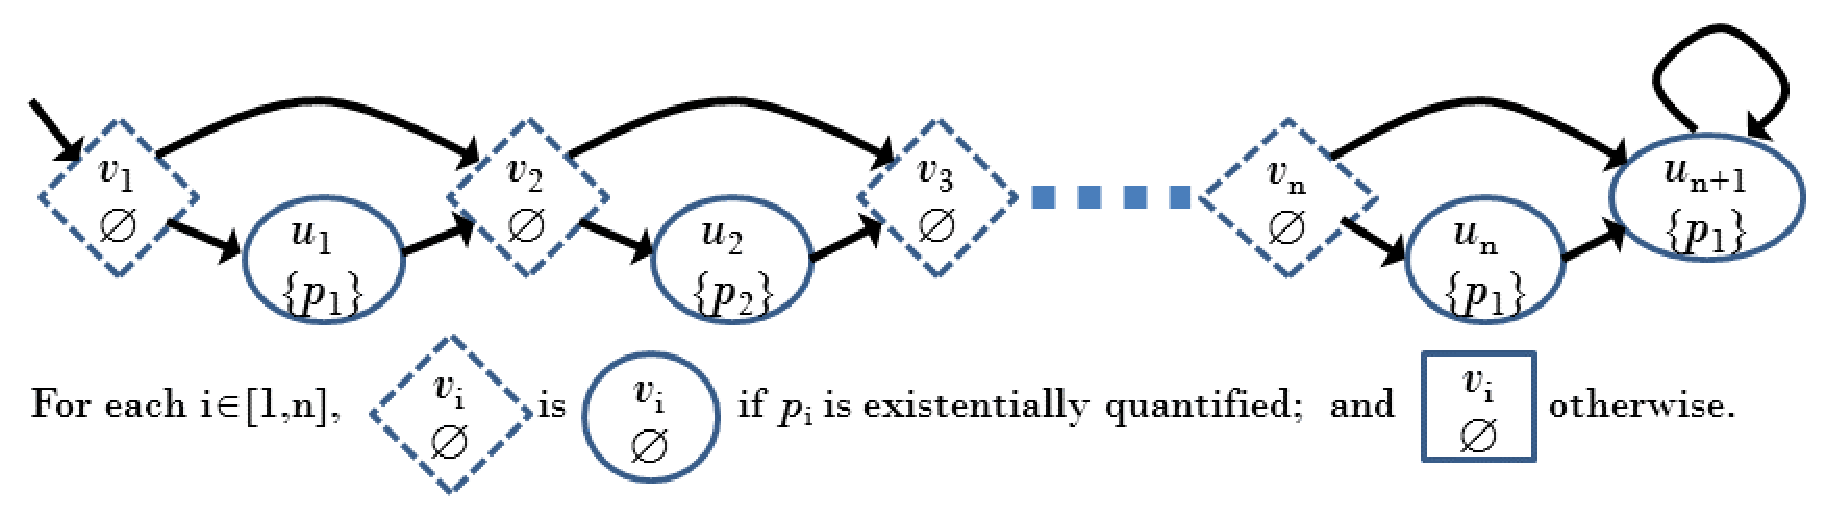
\epsfig{file=gg.altp.eps,width=150mm} 
% \input{gg.atlp.psp80.tex}
\\
$\bigcirc$ belongs to Agent 1 and $\pfrr$ belongs to Agent 2.
\end{center}
\caption{Game graph for the PSPACE-hardness proof of a Boolean formula
with $n$ propositions}
\label{fig.gg.bsil.nphard}
\end{figure}

In the graph, we use oval nodes for states owned by Agent 1 and 
square nodes for states owned by Agent 2.
In each state, we put down its name and the set of atomic
propositions that are true at the node.
For each atomic proposition $p_i\in P$,
we have a corresponding subgraph consisting of nodes
$v_i$ and $u_i$.
The subgraph of $u_i$ corresponds to $\Gamma_{p_i}$ and
and that of $v_i,u_i$ together corresponds to $\Omega_{p_i}$.  

The design of the graph allows only at most one visit
to states $v_1,\ldots,v_n$.
For all $i\in[1,n]$, state $v_i$ is owned by Agent 2 if $p_i$ is
universally quantified;
and owned by Agent 1 otherwise.
If $p_i$ is owned by Agent 1,
then Agent 1 can choose either
$(v_i,u_i)$ or $(v_i,v_{i+1})$.
If $p_i$ is owned by Agent 2,
then both choices of Agent 2 at node $v_i$ must yield
satisfaction of $\eta$.

We construct an ATL$^+$ formula $\phi_\eta$
as % follows.
% \begin{center}
$\langle 1\rangle \bigwedge_{1\leq i\leq k}
\bigvee_{1\leq j\leq h_k} \tau(l_{i,j})$ 
% \end{center}
where $\tau(p)\defn \pevt p$ and $\tau(\neg p)\defn \pfrr \neg p$. 
I.e., $\phi_\eta$ is obtained from $\eta$ by replacing the leading quantifiers in $\eta$ by $\langle 1 \rangle$.

We now show that $\calg_\eta \models \phi_\eta$ if, and only if, $\eta$ is satisfied (i.e., if $\eta$ is a tautology).
The  latter is the case if there is a winning strategy for a `satisfier' in the following game between a `satisfier' and a `refuter':
following the order of the bound variables, the `satisfier' and `refuter' choose the truth value of the existentially and universally bound variables, respectively.
When all variables are assigned truth values, the `satisfier' wins if the CNF formula is satisfied with these values. Otherwise, the refuter wins.

Taking a winning strategy of the satisfier in this game obviously provides a winning strategy for Agent 1 and, vice versa, a winning strategy of Agent 1 in the model-checking game can be used as a winning strategy for the `satisfier' in the satisfaction game.
\qed

We have an example for the reduction in the proof 
of Lemma~\ref{lemma.bsil.mck.nphard}.  

{\example \label{exmp.bsil.nphard}:}
Given
$\eta\equiv \exists p\forall q\exists r
((p\vee q \vee r)\wedge(\neg p \vee \neg r))$,
according to the construction
in the proof of Lemma~\ref{lemma.bsil.mck.nphard},
we have the following ATL$^+$ formula:
$\phi_\eta\defn 
\langle1\rangle(((\pevt p)\vee (\pevt q) \vee (\pevt r))
  \wedge((\pfrr\neg p) \vee (\pfrr\neg r)))$.
\qed

Following Lemmas~\ref{lemma.bsil.mck.nphard} and
\ref{lemma.alg.pspace}, we obtain the complexity of our model-checking problems.

{\lemma\label{lemma.bsil.pspace.complete} The BSIL and ATL$^+$ model-checking
problems are PSPACE-complete.
} \qed


